 %-----------------------------------------------------------
% Bagian Utama Laporan Tugas Akhir
%------------------------------------------------------------


% Tipe dokumen adalah report dengan satu kolom kertas A4 satu sisi.

% Ukuran font 12 pt
\documentclass[12pt, a4paper, onecolumn, oneside, final, table]{report}

% Load konfigurasi LaTeX untuk tipe laporan Tugas Akhir
\usepackage{ta}
\usepackage{tikz}
\usepackage{amsmath}
\usepackage{longtable}
\usepackage{tabularx}
\usepackage{cite}
\usepackage{appendix}
\usepackage{xcolor}
% \usetikzlibrary{matrix,backgrounds}
% \usepackage{pgfplots}
% \pgfplotsset{compat=1.16}
\renewcommand\appendixname{Appendices}
\renewcommand\appendixpagename{Appendices}
\renewcommand\appendixtocname{Appendices}
\newcommand{\ignore}[1]{}
% tambahan
\usepackage[T1]{fontenc}
\usepackage[utf8]{inputenc}
\usepackage{textcomp}
\usepackage{mathtools,mathptmx}
\usepackage{listings}
\usepackage{xcolor}
\usepackage{braket}
\usepackage{bigints}
\DeclareUnicodeCharacter{2212}{-}
\usetikzlibrary{intersections,positioning,arrows.meta,shapes.geometric,fit,calc}
\definecolor{codegreen}{rgb}{0,0.6,0}
\definecolor{codegray}{rgb}{0.5,0.5,0.5}
\definecolor{codepurple}{rgb}{0.58,0,0.82}
\definecolor{backcolour}{rgb}{0.95,0.95,0.92}

\lstdefinestyle{mystyle}{
    commentstyle=\color{codegreen},
    keywordstyle=\color{magenta},
    numberstyle=\scriptsize\color{codegray},
    stringstyle=\color{codepurple},
    basicstyle=\ttfamily\scriptsize,
    breakatwhitespace=false,         
    breaklines=true,                 
    captionpos=b,                    
    keepspaces=true,                 
    numbers=left,                    
    numbersep=10pt,                  
    showspaces=false,                
    showstringspaces=false,
    showtabs=false,                  
    tabsize=2
}

\lstset{style=mystyle}
\usepackage{pdfpages}
%\usepackage[table,xcdraw]{xcolor}

% Pengaturan pemenggalan kata / hyphenation
\hyphenation{dengan di-mo-del-kan mo-du-la-si Nu-me-ro-logy Pe-ne-ra-pan di-nya-ta-kan}

% Load konfigurasi khusus untuk laporan yang sedang dibuat
\input{konfigurasi}

% Awal bagian penulisan laporan Tugas Akhir
\begin{document}

% Sampul Laporan Tugas Akhir
\include{sampul}

% Tidak mengaktifkan penomoran halaman
\pagenumbering{gobble}

% Halaman Pengesahan
% \addChapter{APPROVAL PAGE}
% \include{pengesahan}

% Halaman Pernyataan Orisinalitas
% \addChapter{SELF DECLARATION AGAINST PLAGIARISM}
% \include{orisinalitas}

% Menggunakan penomoran halaman Romawi
\pagenumbering{roman}

% Setelah bagian ini, halaman dihitung sebagai halaman ke-2
\setcounter{page}{1}

% Abstrak dalam Bahasa Indonesia
%\addChapter{ABSTRAK}
%%-----------------------------------------------------------------------------
% Abstrak (Bahasa Indonesia)
%-----------------------------------------------------------------------------


\chapter*{Abstrak}

	Penelitian ini mengembangkan sistem berbasis \textit{cloud} berbiaya rendah untuk mendeteksi kesiapan panen padi, dirancang bagi petani gurem dan divalidasi pada skala \textit{bench} dengan empat tanaman \textit{polybag} di dalam satu \textit{litter box}. Sistem menyasar dua kesenjangan: ketidaksesuaian biaya pencitraan satelit dan wahana udara tanpa awak pada skala sub-hektare, serta keterbatasan \textit{closed-world} pengklasifikasi terlatih yang tetap memberi label fenologi pada citra non-padi atau yang tidak layak ditafsirkan. Modul ESP32-CAM AI-Thinker dengan sensor OV3660 menangkap satu citra kanopi dari atas pada tiap bangun \textit{deep-sleep} dan mengunggahnya melalui Google Cloud Storage ke layanan Flask di Google Cloud Run, yang menuliskan prediksi ke Firebase \textit{Realtime Database} untuk dasbor \textit{Progressive Web App} yang ditempatkan di Netlify. Empat keluarga klasifikasi dibandingkan pada dataset terkurasi 1140 citra (1036 untuk validasi silang \textit{stratified 5-fold}, 104 sisanya \textit{held-out test}) yang mencakup fase vegetatif, generatif, dan matur: \textit{machine learning} klasik atas indeks vegetasi warna dengan fitur tekstur \textit{Gray Level Co-occurrence Matrix}, \textit{backbone} konvolusional \textit{transfer learning}, \textit{hybrid late-fusion}, dan \textit{endpoint vision-language} yang dipakai sebagai penjaga gerbang \textit{open-world}, bukan pengklasifikasi utama. Konfigurasi \textit{hybrid} EfficientNetB0 dengan fitur ExGR memimpin Macro F1 uji pada 0.9662 dan \textit{Support Vector Machine} klasik dengan ExGR menyusul di 0.9577 dengan artefak 55 KB, tetapi kesetaraan ini tidak terbawa ke sensor ESP32-CAM yang di-\textit{deploy}, sehingga \textit{pipeline} tetap memakai pengklasifikasi \textit{hybrid}. Penjaga gerbang \textit{vision-language} yang di-\textit{deploy} (Gemini 2.5 Flash Lite) menolak seluruh dua belas citra non-padi pada \textit{false-accept rate} 0 persen dan \textit{false-reject rate} 4.81 persen, dengan latensi \textit{end-to-end} bermedian 8.57 detik, jauh di bawah jadwal pengambilan citra tiap sepuluh menit. Tata kelola data ditanam langsung ke dalam arsitektur melalui residensi penyimpanan di wilayah Indonesia, pemisahan identitas perangkat dan petani, kontrol akses \textit{Identity and Access Management} \textit{least-privilege}, serta jejak audit yang selaras dengan Undang-Undang Nomor 19 Tahun 2016 tentang Informasi dan Transaksi Elektronik, Peraturan Pemerintah Nomor 71 Tahun 2019, Undang-Undang Nomor 27 Tahun 2022 tentang Pelindungan Data Pribadi, ISO/IEC 30141:2024, dan Rekomendasi ITU-T Y.2060.\\
\\
\textbf{Kata kunci:} fenologi padi, pencitraan proksimal, ESP32-CAM, \textit{vision-language model}, \textit{open-set recognition}, tata kelola data IoT, pertanian rakyat.

%-----------------------------------------------------------------------------


% Abstrak dalam Bahasa Inggris
\addChapter{ABSTRACT}
%---------------------------------------------------------
% Abstrak (Bahasa Inggris)
%---------------------------------------------------------
\chapter*{Abstract}
\vspace*{0.7cm}

\noindent This study develops a low-cost cloud-based system for rice harvest-readiness detection, designed for smallholder plots and validated at bench scale on four polybag-grown plants inside a single litter box. It targets two gaps: the cost mismatch of satellite and unmanned-aerial-vehicle sensing at sub-hectare scale, and the closed-world limitation of supervised classifiers that label non-rice or unusable frames. An ESP32-CAM AI-Thinker module with an OV3660 sensor captures a top-down canopy image on each deep-sleep wake and uploads it through Google Cloud Storage to a Flask service on Google Cloud Run, which writes predictions into a Firebase Realtime Database for a Netlify-hosted Progressive Web App dashboard. Four classification families are compared on the same 1140-image curated dataset (1036 for five-fold stratified cross-validation, 104 held-out test) across vegetative, generative, and mature phases: classical machine learning over color vegetation indices with Gray Level Co-occurrence Matrix texture, transfer-learned convolutional backbones, late-fusion hybrids, and hosted vision-language endpoints used as open-world gatekeepers rather than primary classifiers. The hybrid EfficientNetB0 with ExGR leads test Macro F1 at 0.9662 and the classical Support Vector Machine with ExGR follows at 0.9577 in a 55 KB artifact, but this parity does not carry to the deployed ESP32-CAM sensor, so the pipeline retains the hybrid classifier. The deployed gatekeeper (Gemini 2.5 Flash Lite) rejects all twelve non-rice probes at a 0 percent false-accept and 4.81 percent false-reject rate, with 8.57 second median end-to-end latency within a ten-minute capture cadence. Data governance is encoded into the architecture through Indonesia-region storage residency, separation of device and farmer identifiers, least-privilege Identity and Access Management, and audit logging aligned with Law Number 19 of 2016 on Electronic Information and Transactions, Government Regulation Number 71 of 2019, Law Number 27 of 2022 on Personal Data Protection, ISO/IEC 30141:2024, and ITU-T Recommendation Y.2060.
\vspace{0.2in}
 \noindent
\\ \textbf{Keywords:} rice phenology, proximal imaging, ESP32-CAM, vision-language model, open-set recognition, IoT data governance, smallholder agriculture.

%------------------------------------------------------------


% Ucapan Terima Kasih
% \addChapter{ACKNOWLEDGMENTS}
% \include{ucapan}

% Kata Pengantar
% \addChapter{\kataPengantar}
% \include{pengantar}

% Daftar Isi
\tableofcontents
\clearpage

% Daftar Gambar
\listoffigures
\clearpage

% Daftar Tabel
\listoftables
\clearpage

% Daftar Singkatan / List of Abbreviations
\addChapter{LIST OF ABBREVIATIONS}
\include{singkatan}

% Daftar Achievement
%\addChapter{ACHIEVEMENT}
%\include{achievement}

% Menggunakan penomoran Arab (1, 2, 3, ...)
\pagenumbering{arabic}

% Bab 1: Pendahuluan
%-----------------------------------------------------------------------------
\chapter{\babSatu}
%-----------------------------------------------------------------------------
% Chapter 1 menceritakan gambaran singkat dari penelitian. Penjelasan lebih rinci-nya nanti di Chapter 2, 3, 4, dll. Yang pertama disusun adalah Chapter 2 dan Chapter 3 dulu, tulis semua informasi terkait yang berhasil dihimpun, baru maju ke Chapter 1. Harus bisa menjawab semua pertanyaan yang mungkin ditanyakan.
 


%-----------------------------------------------------------------------------
\section{Background}

%----------------------------------------------------------------------------
Rice (\textit{Oryza sativa} L.) is one of the world's most essential staple food crops, vital for the food security of more than half of the global population, with Asia accounting for the dominant share of global production and consumption \cite{mohidem2022rice}. In Indonesia, the 2023 Agricultural Census reports that 17{,}251{,}432 of 27{,}802{,}434 agricultural land users (about 62 percent) are smallholder farmers (\textit{petani gurem}) cultivating less than 0.5 hectares, with food crops forming the dominant subsector at 15{,}550{,}786 farming households \cite{bps2023sensus}. For these farmers, harvest timing is decisive for both yield quality and income: harvesting too early reduces yield and produces immature grains with elevated chalkiness, while delayed harvesting in tropical regions lowers the head rice rate and increases shattering losses, both degrading milling quality and market value \cite{zhou2025metaharvest}. Accurate identification of rice phenological stages, especially the transition into the mature, harvest-ready phase, is therefore critical for sound agronomic decisions on smallholder plots.

In practice, smallholder farmers in Indonesia rely on Days After Sowing (DAS) estimation or visual inspection to decide harvest timing. These methods are imprecise because growth phase duration varies with cultivar and microclimatic conditions such as temperature, leading to inconsistent decisions and avoidable post-harvest losses \cite{sanwong2023ricetemp}. The problem is amplified on small plots, where access to agronomic expertise and continuous monitoring is limited.

Precision agriculture has introduced remote sensing technologies such as satellite imagery and Unmanned Aerial Vehicle (UAV) mounted multispectral cameras, which monitor crop development through vegetation indices like the Normalized Difference Vegetation Index (NDVI) \cite{huang2021ndvi}. These technologies correlate strongly with crop phenology, but their acquisition cost, recurring operational expense, and required technical expertise place them out of reach for smallholder farmers \cite{boursianis2022iot}. This leaves a clear gap: affordable proximal (in-field) monitoring solutions that can be deployed with minimal infrastructure and operated without specialized skills.

Low-cost embedded imaging modules offer a viable pathway. The ESP32-CAM, an inexpensive system-on-chip integrating a camera sensor with a Wi-Fi microcontroller, can be deployed in the field for close-range, top-down rice canopy capture \cite{elhattab2023esp32cam}. Paired with a cloud backend, it forms an Internet of Things (IoT) monitoring system suited to resource-constrained settings. Field images from consumer-grade sensors, however, exhibit complex backgrounds with variable illumination, motion blur, and inadvertent capture of non-rice objects \cite{tan2023riceres2net}, all of which require a robust validation step before reliable interpretation.

Once a usable canopy image is available, the choice of classification approach is not obvious. Classical machine learning trained on hand-crafted vegetation indices and Gray Level Co-occurrence Matrix (GLCM) texture descriptors offers interpretable, low-resource inference. Transfer-learning Convolutional Neural Networks (CNNs) have achieved high accuracy on crop classification in controlled settings \cite{qin2023ricephenology,tan2023riceres2net}. Hybrid architectures fuse a CNN backbone with hand-crafted vegetation features at the classification head, combining deep representations with an agronomic prior. Large Language Models (LLMs) and Vision-Language Models (VLMs) such as the GPT-4o and Gemini families have demonstrated strong zero-shot generalization across visual recognition tasks without task-specific training \cite{zhang2024vlmsurvey}. Each family occupies a different point in the accuracy, latency, cost, and data-requirement design space, yet no systematic head-to-head comparison of the four for rice harvest-readiness detection from low-cost in-field imaging is available in the literature.

Conventional supervised classifiers operate under a closed-world assumption: they assign every input to one of the predefined classes regardless of relevance. In an open field, where the camera may capture soil, water, equipment, or other out-of-distribution objects, such classifiers produce confident but spurious harvest-readiness predictions that erode system reliability \cite{geng2021openset}. Evidence on VLMs in agricultural visual recognition is nuanced: zero-shot performance has been demonstrated on tasks such as weed detection, but accuracy and interpretability are materially shaped by prompt construction rather than raw model capacity alone, which leaves VLMs short of supervised baselines as primary classifiers in the agricultural domain \cite{frontiers2026weedvlm}. This motivates a defensive design in which the VLM serves as a gatekeeper that verifies whether an input genuinely contains rice and is of acceptable quality, rather than the primary phenology classifier. Pairing such a gatekeeper with the strongest supervised classifier addresses both the open-world limitation and the scarcity of labelled rice canopy imagery.

Beyond the technical dimension, an IoT-based agricultural monitoring system transmits, stores, and processes digital data across telecommunication networks, placing it within the scope of national and international data governance frameworks. In Indonesia, Law Number 19 of 2016 on Electronic Information and Transactions establishes the legal basis for secure handling of electronically transmitted data \cite{uuite2016}, while Government Regulation Number 71 of 2019 on the Implementation of Electronic Systems and Transactions sets reliability, security, and accountability requirements for electronic system operators \cite{pp71_2019}. Law Number 27 of 2022 on Personal Data Protection further establishes the first comprehensive personal data protection regime in Indonesia, with direct implications for farmer-side identifiers handled by the dashboard \cite{uupdp2022}. Internationally, ISO/IEC 30141:2024 defines an IoT reference architecture emphasizing interoperability, security, and trustworthiness \cite{iso30141_2024}, and ITU-T Recommendation Y.2060 outlines the foundational characteristics of IoT including network interconnectivity and embedded security \cite{itut_y2060}. From the perspective of telecommunication regulation and management, aligning an affordable agricultural IoT platform with these frameworks is essential for responsible, scalable, and sustainable adoption.


%--------------------------------------------------------
\section{Problem Identification}
%--------------------------------------------------------
This study is motivated by the following problem statements:
\begin{enumerate}
    \item Harvest-readiness assessment on smallholder rice plots still relies on subjective visual judgment, while satellite, drone, and multispectral approaches do not fit the cost and scale of individual smallholder land.

    \item Conventional supervised classifiers operate under a closed-world assumption, so they force a phenology class onto non-rice objects, blurred frames, or out-of-distribution inputs captured under uncontrolled field conditions.

    \item Publicly available rice-phenology image datasets are scarce, and zero-shot Vision-Language Models cannot be assumed to replace supervised classifiers because they exhibit systematic class-pair confusion at the Generative-to-Mature transition and unstable carry-over to proximal field imagery, even when their headline accuracy on curated benchmarks is competitive.

    \item No systematic comparative evidence exists on which classification family, namely classical machine learning, transfer-learning CNN, hybrid CNN with vegetation index features, or Vision-Language Models, best balances classification performance, inference latency, and operational cost for rice harvest-readiness detection from low-cost in-field imaging.

    \item Low-cost agricultural IoT prototypes rarely address the data-governance and regulatory obligations that apply once images are transmitted, stored, and processed in the cloud.
\end{enumerate}


\section{Objective and Contributions}
The objectives and contributions of this study are as follows:
\begin{enumerate}
    \item To develop an ESP32-CAM in-field imaging subsystem that captures rice canopy images on a periodic deep-sleep wake cycle and delivers them to a cloud backend with a dashboard, providing an affordable alternative to satellite, drone, and multispectral monitoring on smallholder plots.

    \item To conduct a systematic comparative study of four classification families, namely classical machine learning with vegetation indices and GLCM texture features, transfer-learning Convolutional Neural Networks, hybrid CNN with vegetation index features, and Vision-Language Models, on classification performance, inference latency, and operational cost for rice harvest-readiness detection.

    \item To integrate a tiered detection pipeline consisting of a Vision-Language Model open-world gatekeeper and a phenology classifier covering three stages, namely vegetative, generative, and mature.

    \item To use the Vision-Language Model as a gatekeeper rather than as the primary classifier, rejecting non-rice and low-quality inputs in order to mitigate the closed-world limitation of supervised classifiers and the scarcity of labelled rice imagery.

    \item To examine the data-governance and regulatory requirements that apply to the cloud-based imaging pipeline and to align the system design with recognized electronic-system, data-protection, and IoT reference-architecture principles.
\end{enumerate}


%--------------------------------------------------------
\section{Scope of Work}
%--------------------------------------------------------
The scope of this study includes:
\begin{enumerate}
    \item The imaging hardware is limited to a single low-cost ESP32-CAM (AI-Thinker, OV3660) mounted above a bench-scale rice plant setup consisting of four polybags placed inside a litter box, configured for close-range, top-down, periodic deep-sleep wake-cycle capture. Other camera types, continuous video recording, and additional sensors or actuators are outside this scope.

    \item The detection target is rice phenology classified into three stages only, namely vegetative, generative, and mature, where mature denotes harvest readiness. Other crops, diseases, pests, and yield estimation are not covered.

    \item The detection pipeline is limited to two tiers, namely a Vision-Language Model open-world gatekeeper and a phenology classifier. The Vision-Language Model is used for input rejection and gatekeeping, not as the primary stage classifier.

    \item The comparative study covers four classification families, namely classical machine learning with vegetation indices and GLCM texture features, transfer-learning Convolutional Neural Networks, hybrid CNN with vegetation index features, and Vision-Language Models. Each family is represented by a small set of implementations rather than an exhaustive survey, and is evaluated on classification performance, inference latency, and operational cost.

    \item Training and offline evaluation use a dataset curated by the author from publicly available rice imagery on Hugging Face and Roboflow, with manual organization and three-class labelling. No primary dataset is collected for model training. Field validation with the ESP32-CAM is performed on the bench-scale polybag setup and is limited to verification of the mature stage as a proof-of-concept deployment, not a statistical validation of all three classes in an actual smallholder field.

    \item All model inference runs on the cloud backend, consisting of Google Cloud Run, Google Cloud Storage, and Firebase Realtime Database, with a Progressive Web Application dashboard hosted on Netlify. On-device or edge deployment on the ESP32-CAM or other boards is outside this scope, and deployment is at prototype scale on the bench-scale polybag setup rather than at full production or large-area operation.

    \item The data-governance analysis is limited to applicable Indonesian electronic-system and data-protection regulations and recognized IoT reference architectures. It is a design-alignment review, not a legal audit or formal compliance certification.
\end{enumerate}



%--------------------------------------------------------
\section{Research Methodology}
%--------------------------------------------------------
This study is divided into several Work Packages (WP) to support structured execution and ensure alignment with the intended objectives. The following WPs will be carried out:
\begin{itemize}

    \item WP 1: Research Identification \\
    Identify the technical challenges in detecting rice harvest readiness from low-cost in-field imagery, including the subjectivity of manual visual judgment commonly used by smallholder farmers, the cost and scale mismatch of remote sensing approaches for individual smallholder plots, the closed-world limitation of conventional supervised classifiers, the scarcity of labelled rice canopy imagery, and the absence of systematic comparative evidence across classification families.

    \item WP 2: Literature and Regulatory Study \\
    Review recent research on proximal (in-field) crop imaging, rice phenology classification, open-set recognition, and the use of Vision-Language Models for zero-shot agricultural tasks. Review the Indonesian regulatory framework (Law Number 19 of 2016, Government Regulation Number 71 of 2019, and Law Number 27 of 2022 on Personal Data Protection) and international references such as ISO/IEC 30141 and ITU-T Recommendation Y.2060 on IoT reference architecture.

    \item WP 3: System Design and Deployment \\
    Develop the proposed system architecture by mounting a low-cost ESP32-CAM (AI-Thinker, OV3660) above a bench-scale rice plant setup of four polybags placed inside a litter box for close-range, top-down, periodic deep-sleep wake-cycle capture, deploying a Flask backend on Google Cloud Run, and configuring Google Cloud Storage, Firebase Realtime Database, and the Progressive Web Application dashboard together with the supporting network connectivity.

    \item WP 4: Dataset Curation and Preprocessing \\
    Curate a three-class rice phenology dataset from publicly available rice imagery on Hugging Face and Roboflow, with manual organization and labelling into vegetative, generative, and mature classes. Apply standard image preprocessing such as resizing and normalization, and partition the data for five-fold cross-validation on the training portion and a held-out test set.

    \item WP 5: Model Development and Comparative Study \\
    Implement and compare four classification families, namely classical machine learning with vegetation indices and GLCM texture features, transfer-learning Convolutional Neural Networks, hybrid CNN with vegetation index features at the classification head, and Vision-Language Models. Integrate the best-performing supervised classifier with the Vision-Language Model open-world gatekeeper into the production pipeline with dashboard visualization.

    \item WP 6: Evaluation, Compliance, and Reporting \\
    Evaluate classification performance on the held-out test set, gatekeeper rejection behavior on out-of-distribution inputs, inference latency, and operational cost on the cloud backend. Verify the integrated pipeline through a proof-of-concept ESP32-CAM deployment on the bench-scale polybag setup limited to the mature stage. Conduct a data-governance and compliance assessment against the relevant national regulations and international IoT references, and document findings in the final thesis report.
\end{itemize}

%-----------------------------------------------------------------------------
%\section{Organization of the Thesis}
%-----------------------------------------------------------------------------
%The rest of this thesis is organized as follows:
%\begin{itemize}
%\item[] \textbf{CHAPTER II: \babDua}\\
%This chapter provides basic concepts used in this thesis. The explanation focuses on general quantum communications and the basic concept of OAM, qudit, multiplexing in classical and quantum communications.  
%\item[] \textbf{CHAPTER III: \babTiga}\\
%This chapter describes the system model, %including parameters used in the proposal %thesis. 
% research methodology, and research design.	
% \item[] \textbf{CHAPTER 4: \babEmpat}\\
% This chapter discusses the result of this thesis, starting from the validation and observation to the performance of the proposed design. Then, BER, capacity and spectral efficiency are used to analyze the performance of the proposed codes.
% \item[] \textbf{CHAPTER 5: \babLima}\\
% This chapter provides the conclusion of this thesis and notifies the future works.
%\end{itemize}

\section{Research Plan and Action Point}

This study will be conducted in a structured manner following a predetermined schedule to ensure timely completion and alignment with the planned targets. Table~\ref{tab:tabel1-1} presents an overview of the workflow, including the stages and activities to be carried out throughout its duration.

\begin{table}[h]
    \centering
    \caption{Thesis Schedule}
    \label{tab:tabel1-1}
    \small
    \setlength{\tabcolsep}{4pt}
    \renewcommand{\arraystretch}{1.2}
    \begin{tabular}{|p{5.3cm}|c|c|c|c|c|c|c|c|}
        \hline
        \multirow{2}{*}{\textbf{Thesis Component}} & \multicolumn{8}{c|}{\textbf{2026}} \\
        \cline{2-9}
         & \textbf{Jan} & \textbf{Feb} & \textbf{Mar} & \textbf{Apr} & \textbf{May} & \textbf{Jun} & \textbf{Jul} & \textbf{Aug} \\
        \hline
        Research Identification & \cellcolor{green!30} & \cellcolor{green!30} & & & & & & \\
        \hline
        Literature and Regulatory Study & \cellcolor{green!30} & \cellcolor{green!30} & \cellcolor{green!30} & \cellcolor{green!30} & & & & \\
        \hline
        Background Writing & & \cellcolor{green!30} & \cellcolor{green!30} & & & & & \\
        \hline
        Problem Formulation and Objectives & & \cellcolor{green!30} & \cellcolor{green!30} & & & & & \\
        \hline
        System Design and Deployment & & & \cellcolor{green!30} & \cellcolor{green!30} & \cellcolor{green!30} & & & \\
        \hline
        Dataset Curation and Preprocessing & & & \cellcolor{green!30} & \cellcolor{green!30} & & & & \\
        \hline
        Model Development and Comparative Study & & & & \cellcolor{green!30} & \cellcolor{green!30} & \cellcolor{green!30} & & \\
        \hline
        Bench-scale ESP32-CAM Validation & & & & & & \cellcolor{green!30} & \cellcolor{green!30} & \\
        \hline
        Data Governance and Compliance Review & & & & & \cellcolor{green!30} & \cellcolor{green!30} & & \\
        \hline
        Result and Discussion Writing & & & & & \cellcolor{green!30} & \cellcolor{green!30} & \cellcolor{green!30} & \\
        \hline
        Conclusion and Recommendations & & & & & & & \cellcolor{green!30} & \cellcolor{green!30} \\
        \hline
        Thesis Draft Review and Revisions & & & & & & & \cellcolor{green!30} & \cellcolor{green!30} \\
        \hline
        Thesis Seminar and Defense & & & & & & & & \cellcolor{green!30} \\
        \hline
    \end{tabular}
\end{table}



% Bab 2: Konsep Dasar
%-----------------------------------------------------------------------------
\chapter{\babDua}

%------------------------------------------------------------

\section{Rice}
\label{sec:rice}

Rice (\textit{Oryza sativa} L.) is a staple food for more than half of the world's population, with Asia accounting for the dominant share of global production and consumption \cite{mohidem2022rice}. In Indonesia, the 2023 Agricultural Census reports that 17{,}251{,}432 of 27{,}802{,}434 agricultural land users, about 62 percent, are smallholder farmers cultivating less than 0.5 hectares, and food crops including rice form the dominant subsector with 15{,}550{,}786 farming households \cite{bps2023sensus}. Any technological intervention for rice productivity must therefore remain affordable, easy to operate, and deployable on sub-hectare plots that fall well below the scale of industrial precision agriculture.

The rice life cycle is conventionally divided into three growth phases, vegetative, reproductive, and ripening, with a complete cycle of 70 to 170 days depending on cultivar \cite{mohapatra2025staging}. The vegetative phase covers germination, tillering, and leaf development, during which biomass accumulates and the canopy closes. The reproductive phase, also called the generative phase, starts with panicle initiation and continues through booting, heading, and flowering. The ripening phase covers grain filling and maturation, during which starch is translocated to the grains and the canopy senesces toward harvest. This study uses the simplified labels vegetative, generative, and mature, where mature corresponds to the ripening phase and denotes the harvest-ready state.

The transition into the mature phase is the most operationally critical because it determines the harvest window. A meta-analysis of harvest-time effects on rice yield and quality shows that early harvesting reduces yield and produces chalky immature grains, while delayed harvesting in tropical regions lowers the head rice rate and increases shattering losses \cite{zhou2025metaharvest}. Phase boundaries are not rigid in calendar time. Controlled experiments on three rice varieties showed that elevated temperature significantly alters phenological intervals and reduces yield even within the same cultivar \cite{sanwong2023ricetemp}, and China's seasonal rice calendar exhibited measurable shifts in transplanting, heading, and maturity dates between 2003 and 2022 \cite{li2024chinaricecalendar}. A fixed Days After Sowing schedule cannot reliably indicate the harvest moment for every plot, and visual judgment of phase transitions, while accessible to smallholder farmers, is subjective and prone to inter-observer variability.

These characteristics motivate the technical scope of this study. Classifying phenology into vegetative, generative, and mature aligns the recognition task with the actual decisions smallholder farmers must take, especially identifying the harvest-ready state. Because phase transitions are continuous and visually subtle, an on-demand automated system gives a more consistent assessment than periodic manual inspection. The dominance of sub-hectare landholdings also requires the monitoring solution to be low in hardware and operating cost, and free from specialized expertise.

\section{Proximal Imaging}
\label{sec:proximal_imaging}

Crop sensing technologies are grouped by the proximity of the sensor to the canopy. Remote sensing platforms such as satellite constellations and Unmanned Aerial Vehicles (UAVs) observe fields from tens of meters to several hundred kilometers with spatial resolutions from ten meters down to centimeters, but at the cost of platform mobilization expense and dependence on atmospheric conditions. Proximal sensing places sensors within centimeters to a few meters of the plants and provides real-time, ground-level measurements without those dependencies \cite{mezera2021proximalremote}. A direct comparison in winter wheat across four growing seasons showed that proximal on-the-go sensors remain operable under cloud cover that prevents reliable satellite acquisition, a recurring constraint during critical phenological transitions \cite{mezera2021proximalremote}.

For rice, proximal imaging with consumer-grade Red-Green-Blue (RGB) cameras is a low-cost alternative to multispectral remote sensing platforms that remain underutilized in smallholder contexts. A study covering more than 4{,}800 harvesting plots across six countries showed that vertically downward RGB images of the rice canopy at 0.8 to 0.9 meter, resolved over one square meter consistent with FAO harvesting standards, support accurate yield estimation without labor-intensive crop cuts \cite{tanaka2023rgbrice}. The same study framed proximal RGB imaging as a practical pathway for rice monitoring in the global South, where smallholder land structure makes large-area remote sensing economically unattractive.

This study follows the same proximal RGB principle. A single consumer-grade RGB camera is mounted statically above the rice canopy for close-range, top-down, on-demand capture, rather than continuous video or oblique handheld photography. The static top-down arrangement constrains the geometric variability of the field of view, and the on-demand trigger makes bandwidth, storage, and inference cost scale with farmer interaction rather than sensor duty cycle. The setup trades spatial coverage of UAV or satellite sensing for plot-level temporal flexibility and operational simplicity.

Proximal RGB imaging in the field is not without challenges. Cameras must operate under uncontrolled illumination, and ground-based rice yield studies report that imaging time of day measurably affects color balance and contrast \cite{tanaka2023rgbrice}. Motion blur from mounting vibration, wind, or platform displacement degrades downstream vision tasks, with controlled experiments showing segmentation accuracy on crop and weed images dropping from a mean intersection-over-union of about 0.80 on sharp images to about 0.63 on motion-blurred ones \cite{yun2023motiondeblurring}. The camera may also capture frames containing soil, equipment, water, or other non-rice content that are uninformative for phenology classification.

A closed-world classifier would assign a phenology label to images that contain no rice canopy or that are otherwise unusable for phenology interpretation, so the inference pipeline carries an open-world rejection step at its entry. A Vision-Language Model gatekeeper enforces this rejection before the supervised classifier receives the frame.

\begin{figure}
    \centering
    \includegraphics[width=0.55\textwidth]{img/Overhead canopy capture.png}
    \caption{Overhead RGB Canopy Capture}
    \label{fig:proximal-imaging}
\end{figure}

\section{ESP32-CAM}

The ESP32-CAM is a compact, low-cost embedded vision module built around the Espressif ESP32 system-on-chip and a camera daughterboard. The ESP32 integrates a dual-core 32-bit microcontroller, several hundred kilobytes of on-chip Static Random Access Memory (SRAM), and integrated 2.4 GHz Wi-Fi and Bluetooth connectivity, which makes it a popular choice for Internet of Things deployments that combine wireless data transport with on-device control \cite{hercog2023esp32iot}. In the AI-Thinker ESP32-CAM variant used in this study, the system-on-chip is paired with 4 MB of external Pseudo Static Random Access Memory (PSRAM) to buffer image frames, 4 MB of Serial Peripheral Interface (SPI) flash for firmware, and a microSD card slot for optional local logging. The full imaging node fits within roughly 27 by 40 millimeters at a unit cost well below ten United States dollars, which is the order of magnitude required for a monitoring solution that smallholder farmers can replicate.

The optical front end is the OmniVision OV3660, a three-megapixel Complementary Metal Oxide Semiconductor (CMOS) sensor that supports capture up to 2048 by 1536 pixels with on-sensor Joint Photographic Experts Group (JPEG) compression. Compared with the OV2640 commonly fitted to default AI-Thinker boards, the OV3660 offers higher native spatial resolution, which is useful for resolving rice canopy texture and panicle morphology at close range. The sensor is driven by the ESP32 over a parallel data interface and an Inter-Integrated Circuit (I2C) control bus, and JPEG-encoded frames are buffered in PSRAM before transmission, so no companion processor is required on the acquisition path.

The ESP32 platform has been adopted as the imaging and sensing endpoint of several plant monitoring systems. Elhattab et al. proposed a remote plant growth monitoring system in which an ESP32-CAM transmits images over Wi-Fi to a mobile application, with the server side handling visualization and growth tracking \cite{elhattab2023esp32cam}. Correa-Quiroz et al. reported a greenhouse system in which an ESP32 microcontroller aggregates climate, soil moisture, and irrigation telemetry and streams them to a cloud dashboard \cite{correaquiroz2025esp32greenhouse}. The same offloading pattern recurs outside agriculture in beehive and fermentation monitoring nodes that forward local measurements to an Internet of Things cloud platform such as ThingSpeak \cite{hercog2023esp32iot}. Across these deployments the ESP32 acts as a capture-and-upload endpoint rather than an inference platform, with analytical workload deferred to a more capable backend. The few hundred kilobytes of SRAM and few megabytes of PSRAM cannot accommodate the parameter footprint of mainstream Convolutional Neural Networks (CNNs) at full precision, and even quantized models leave little headroom for the runtime, the input pipeline, and the JPEG encoder.

In this study, the ESP32-CAM is configured strictly as a periodic image acquisition node. On each wake from a deep-sleep cycle, the device captures a single JPEG frame at full resolution, attaches a timestamp and device identifier, and uploads the frame to cloud storage over Wi-Fi before returning to sleep. The device performs no preprocessing beyond the sensor's built-in pipeline and does not run any classification model locally. This division keeps the embedded firmware small and predictable, concentrates the energy budget on short Wi-Fi bursts rather than continuous inference, and allows classifier updates to be rolled out by changing the cloud service alone.

The hardware choice introduces constraints. The OV3660 lacks the radiometric calibration interfaces of dedicated agricultural cameras, and its automatic exposure and white balance operate on a single integrated RGB Bayer sensor, so any colorimetric analysis downstream is implicitly conditioned on the image signal processor. The static top-down mounting reduces but does not eliminate pose variability, and the on-demand capture mode reduces motion blur compared with continuous video, although ambient illumination changes during the day remain uncontrolled. These constraints are accepted as part of a trade-off that prioritizes hardware affordability over laboratory-grade radiometric fidelity.

\begin{figure}
    \centering
    \includegraphics[width=0.5\textwidth]{img/espcam.png}
    \caption{ESP32-CAM}
    \label{fig:esp32cam}
\end{figure}

\section{Image Features}

In addition to raw pixel intensities, this study uses compact image features derived from each RGB frame as inputs to the classical machine learning classifiers and to the handcrafted branch of the hybrid model. Two families are used in parallel: color vegetation indices from the per-pixel red, green, and blue channels, and Gray Level Co-occurrence Matrix (GLCM) texture descriptors from a grayscale projection of the frame. Color vegetation indices capture chromatic information sensitive to chlorophyll content and canopy greenness, while GLCM descriptors capture the spatial arrangement of intensities that reflects canopy structure. Recent work on cotton yield estimation showed that fusing texture and color features from an RGB sensor outperforms either family alone, raising the coefficient of determination of the yield model to 0.91 on validation data \cite{ma2022cottonRGB}. A similar pattern has been reported for rice canopy estimation from Unmanned Aerial Vehicle (UAV) imagery, where texture features compensate for spectral information at early stages dominated by soil and water background noise and at later stages affected by spectral saturation as the canopy closes \cite{liu2023glcmrice}.

\subsection{Color Vegetation Indices}

Color vegetation indices are analytical combinations of the red, green, and blue channels that emphasize green vegetation against soil, residue, or shadow. They serve as low-cost substitutes for multispectral indices such as the Normalized Difference Vegetation Index (NDVI) when only a consumer-grade RGB camera is available, since they can be computed without a dedicated near-infrared band. Recent RGB-based studies report strong correlations between selected color indices and crop biophysical traits across cereal, cotton, and cover crop systems \cite{ma2022cottonRGB}.

This study uses eight color vegetation indices widely reported in RGB-based precision agriculture: the Excess Green (ExG), Excess Red (ExR), Excess Green minus Excess Red (ExGR), Visible Atmospherically Resistant Index (VARI), Green Leaf Index (GLI), Normalized Green Red Difference Index (NGRDI), Modified Green Red Vegetation Index (MGRVI), and Red Green Blue Vegetation Index (RGBVI) \cite{ma2022cottonRGB}. Let $R$, $G$, and $B$ denote the raw red, green, and blue intensities of a pixel. The eight indices are defined as:

\begin{figure}
    \centering
    \includegraphics[width=0.85\textwidth]{img/Color Vegetation Indices.png}
    \caption{Color Vegetation Indices}
    \label{fig:vi-indices}
\end{figure}

The eight indices fall into two groups. ExG, ExR, and ExGR are difference-style indices that compare a single emphasized channel against the others. ExGR is reported as an effective separator of vegetation from soil and senescent residue because the excess red term suppresses green-red material such as stems and dry tissue that ExG alone tends to misclassify as foliage. NGRDI and MGRVI are ratio-style indices that normalize a green-red contrast against the green-plus-red sum, while GLI normalizes a green-versus-non-green contrast against the full red-green-blue sum, and RGBVI compares the squared green channel against the red-blue product. VARI substitutes blue in the denominator with the opposite sign $(G-R)/(G+R-B)$, which is the atmospheric-resistance correction that gives it robustness against scene-wide haze and brightness changes \cite{ma2022cottonRGB}. Across the rice phenological cycle, the relative proportions of green foliage, panicle, and senescent tissue evolve systematically, so both groups contribute discriminative information for distinguishing the vegetative, generative, and mature phases.

For each RGB frame, the eight indices are computed pixel-wise, and ten descriptive statistics are extracted from each per-index map to form a fixed-length feature vector summarizing the chromatic state of the canopy.

\subsection{GLCM Texture Features}

Color vegetation indices summarize chromatic information at the pixel level but discard the spatial arrangement of intensities. Texture descriptors recover this information by analyzing the statistical relationship between neighboring pixel intensities. The Gray Level Co-occurrence Matrix (GLCM) is a second-order statistical representation that counts the joint occurrence of pixel intensity pairs at a given spatial offset, parameterized by a displacement distance and an angular direction. From a normalized GLCM, scalar descriptors can be derived that capture distinct aspects of local intensity variation.

This study uses four GLCM descriptors widely adopted in GLCM-based crop classification from low-altitude remote sensing imagery: Contrast, Correlation, Energy (also called Angular Second Moment), and Homogeneity \cite{iqbal2021glcmcrop}. Contrast responds to sharp intensity transitions and highlights edge density, while Homogeneity responds inversely and highlights uniform regions. Energy quantifies the textural orderliness of the co-occurrence distribution and increases when the canopy texture is regular. Correlation measures how predictable a neighboring pixel intensity is given the reference pixel and responds to directional structure in the texture. Each descriptor is computed at two pixel offsets of one and three pixels and four angular directions of $0$, $\pi/4$, $\pi/2$, and $3\pi/4$ radians, yielding eight cells per descriptor. The mean and standard deviation across these eight cells are then taken as two summary statistics for that descriptor, so the four descriptors together produce eight texture features that capture both the average textural state and its directional and scale anisotropy.

For the classical machine learning experiments, the eight texture features are concatenated with the ten per-index statistics from each color vegetation index, giving a handcrafted feature vector of eighteen dimensions per vegetation index. The same vector is reused as the handcrafted branch of the hybrid model. Combining texture features with chromatic information is consistent with recent findings that texture compensates for spectral information at early growth stages affected by background interference and at late stages affected by spectral saturation \cite{liu2023glcmrice,ma2022cottonRGB}.

\section{Machine Learning}

The classical machine learning track of this study applies supervised classifiers to the eighteen-dimensional handcrafted feature vector formed by color vegetation index statistics and Gray Level Co-occurrence Matrix descriptors. The motivation is operational: classical classifiers have small parameter counts and low inference cost, which suits a cloud backend that charges per request, and their feature attributions are easier to communicate to non-technical stakeholders. A recent review of machine learning in agriculture confirms that Random Forest, Support Vector Machine, K-Nearest Neighbors, Logistic Regression, and Gradient Boosting remain widely used for crop monitoring, with each method offering a different inductive bias \cite{benos2021ml}. For paddy in particular, Random Forest has been reported to outperform Classification and Regression Trees (CART) and Support Vector Machine on growth phase classification with imbalanced data \cite{suryono2022paddyrf}, the same regime present in the three-class vegetative, generative, and mature partition used here. Five classifiers are evaluated, each covering a distinct inductive family.

\subsection{Random Forest}

Random Forest (RF) is an ensemble of decision trees trained on bootstrap samples, with each split chosen from a random subset of features, and predictions aggregated by majority vote. The construction reduces the variance of a single decision tree, captures non-linear feature interactions, and tolerates heterogeneous feature scales and moderately many irrelevant features. These properties suit the mixed vegetation index statistics and texture descriptors used here, and Random Forest has been reported as a strong classifier for paddy growth phase classification under class imbalance \cite{suryono2022paddyrf}.

\subsection{Support Vector Machine}

Support Vector Machine with a Radial Basis Function kernel (SVM-RBF) constructs a maximum-margin separator in a feature space defined implicitly by a Gaussian kernel, which allows non-linear class boundaries without explicit polynomial expansion. SVM-RBF fits moderate-dimensional tabular vectors well when the sample count is comparable to or larger than the feature dimension, and it is a common baseline in supervised crop monitoring studies \cite{benos2021ml,suryono2022paddyrf}.

\subsection{K-Nearest Neighbors}

K-Nearest Neighbors (KNN) assigns a query point the majority class of its $k$ closest training points under a chosen distance metric, with no parametric training stage. KNN provides a non-parametric, instance-based baseline that is sensitive to the local geometry of the feature distribution and indicates whether the handcrafted feature space admits a simple nearest-neighbor structure aligned with the phenological classes \cite{benos2021ml}.

\subsection{Logistic Regression}

Logistic Regression (LR) fits a linear decision boundary in the input feature space and produces class probabilities through the softmax extension for multiclass problems. As a linear baseline, it indicates whether the handcrafted feature vector is linearly separable across the three phases, which is informative about the geometric difficulty of the task \cite{benos2021ml}.

\subsection{Gradient Boosting}

Gradient Boosting (GB) builds an additive ensemble of shallow decision trees by sequentially fitting each new learner to the residuals of the current ensemble. The stage-wise optimization concentrates capacity on samples that are still misclassified, which is effective on heterogeneous tabular features such as the combined vegetation index and texture descriptors used here \cite{benos2021ml}.

The five classifiers are trained and evaluated on the handcrafted feature vector derived from each of the eight color vegetation indices, producing forty combinations of vegetation index and classifier. All combinations share the same cross-validation protocol so that the contribution of feature choice and the contribution of classifier choice can be isolated.

\section{Deep Learning}

The deep learning track of this study replaces the handcrafted feature pipeline with Convolutional Neural Networks (CNNs) that learn a hierarchy of spatial filters directly from raw pixels. Unlike the vegetation index and Gray Level Co-occurrence Matrix descriptors used in the classical track, CNN filters are trained jointly with the classifier head, so chromatic and structural information are extracted by the same network and optimized for the phenology objective. The cost is a larger parameter count and a stronger dependence on training data volume, which is addressed by transfer learning from networks pretrained on the ImageNet classification dataset. The pretrained backbones provide general-purpose low and mid-level visual features that can be reused for plant imagery after lightweight adaptation, which is the established practice across plant image recognition on small in-field datasets, including rice growth stage classification \cite{pacal2024dlplantdisease,qin2023ricephenology}.

CNN-based recognition of rice growth stages has been demonstrated at both the canopy and the panicle level. Qin et al. trained a ResNet-50 backbone on a six-stage rice phenology dataset of RGB canopy imagery captured across the full life cycle and reported around 87 percent recognition accuracy across the six stages \cite{qin2023ricephenology}. Tan et al. introduced the RiceRes2Net architecture for in-field panicle detection and growth stage recognition and showed that a residual CNN backbone tuned on rice imagery captures fine-grained morphological cues such as panicle emergence and grain filling that are hard to encode by hand \cite{tan2023riceres2net}. These studies establish CNN backbones as a competitive choice for in-field rice phenology recognition and motivate the three backbones evaluated here, selected to span the range from accuracy-oriented designs down to ultra-compact mobile-oriented designs at progressively smaller parameter budgets.

All three backbones are fine-tuned on the curated rice dataset using a two-phase transfer learning protocol. The classification head is first trained with the backbone frozen so that the new softmax weights adapt to the rice feature distribution without disturbing the pretrained filters. The top layers of the backbone are then unfrozen and trained jointly with the head at a lower learning rate to refine high-level features for the target task while preserving the generic low-level filters learned on ImageNet. The same protocol is reused for the visual branch of the hybrid model so that the deep learning and hybrid tracks share their feature extractor under identical training conditions.

\subsection{EfficientNetB0}

EfficientNetB0 is the baseline of the EfficientNet family of CNNs designed through compound scaling, a principled scheme that jointly scales network depth, width, and input resolution under a fixed computational budget \cite{tanle2019efficientnet}. The backbone is built from mobile inverted bottleneck convolutional blocks with squeeze-and-excitation modules and produces a 1280-dimensional embedding from a global average pooling head before the final classification layer \cite{tanle2019efficientnet}. The architecture reaches high ImageNet accuracy with a parameter count of about 5.3 million, which is attractive when classification accuracy is prioritized but the per-request inference cost of a cloud backend still has to remain modest.

In this study, EfficientNetB0 is the primary deep learning backbone for the rice phenology classifier. The ImageNet pretrained weights are reused, the original classification head is replaced by a three-class softmax layer matching the vegetative, generative, and mature labels, and the backbone is fine-tuned on the curated rice dataset. The same backbone is also the visual branch of the hybrid model, so its 1280-dimensional embedding is shared between the deep learning track and the hybrid track and the two pipelines remain directly comparable.

\begin{figure}
    \centering
    \includegraphics[width=0.85\textwidth]{img/EfficientNet-Architecture-diagram.jpg}
    \caption{EfficientNet Architecture}
    \label{fig:effnet-architecture}
\end{figure}

\subsection{MobileNetV2}

MobileNetV2 is a compact CNN backbone originally designed for mobile and embedded deployment, although it is used here as a server-side classifier \cite{sandler2018mobilenetv2}. The architecture is built from inverted residual blocks with linear bottlenecks, in which channel-wise depthwise separable convolutions replace dense spatial convolutions and residual shortcuts connect the low-dimensional bottleneck representations rather than the expanded feature maps \cite{sandler2018mobilenetv2}. The combined effect is a substantial reduction in parameter count, on the order of 3.5 million for the standard configuration, while preserving competitive ImageNet accuracy.

MobileNetV2 enters this study as a lightweight comparison backbone for EfficientNetB0. The same transfer learning protocol is applied, with ImageNet pretrained weights loaded, the classification head replaced by a three-class softmax, and the network fine-tuned on the rice dataset. Its smaller parameter footprint indicates whether the additional capacity of EfficientNetB0 is justified for the three-phase rice phenology task and how much accuracy can be retained when the backbone is sized down toward mobile deployment.

\subsection{MobileNetV3-Small}

MobileNetV3-Small is the most compact configuration in the MobileNetV3 family, designed for execution on devices with very limited compute and memory \cite{howard2019mobilenetv3}. The architecture is the product of Neural Architecture Search combined with the NetAdapt algorithm, and it introduces two changes that distinguish it from the previous MobileNet generation: the h-swish activation, a hardware-friendly approximation of the swish function, and the integration of squeeze-and-excitation modules in selected blocks \cite{howard2019mobilenetv3}. The Small variant carries about 2.5 million parameters and targets latency budgets at which even MobileNetV2 is too costly.

In this study, MobileNetV3-Small is the lightest backbone evaluated and serves as the lower bound on backbone capacity for rice phenology classification. MobileNetV3 has been adopted as a lightweight backbone in related rice agricultural tasks, including pest and disease detection in field imagery, where its low parameter count supports deployment scenarios that EfficientNet-scale models cannot reach \cite{jia2023ricemobilenetv3}. The same two-phase transfer learning protocol used for the other backbones is applied, with ImageNet pretrained weights loaded and the three-class softmax head replacing the original classifier. Inference still runs in the cloud backend, but the small parameter footprint of MobileNetV3-Small benchmarks the lower end of the accuracy versus capacity trade-off relevant for future edge deployment at the sensor node.

\section{Hybrid Model}

The hybrid track combines the learned visual features of a Convolutional Neural Network (CNN) with the handcrafted vegetation index and texture features used in the classical track within a single classifier. The motivation is complementarity: the CNN backbone captures spatial structure and high-level abstraction that pixel-level color statistics and Gray Level Co-occurrence Matrix (GLCM) descriptors cannot represent, while the handcrafted features inject explicit chromatic and textural priors that are aligned with rice canopy biology and were already shown to be informative in the classical track. Recent crop-phenology work has validated that late fusion of CNN-extracted features with handcrafted descriptors improves fine-grained phenological recognition over either family alone, reaching accuracies above 0.92 on crop-specific phenology benchmarks \cite{yang2024phenologynet}.

The architecture used in this study is a late-fusion two-branch network. The visual branch is an EfficientNetB0 backbone with ImageNet pretrained weights and the original classification head removed; its output is reduced by global average pooling to a 1280-dimensional embedding that summarizes the canopy at a high semantic level. The handcrafted branch receives the 18-dimensional feature vector formed by 10 statistics of a single vegetation index map and 8 Gray Level Co-occurrence Matrix texture features computed from the grayscale projection of the same frame, and applies batch normalization to bring the two branches onto comparable scales. The two embeddings are concatenated and passed through a small classification head of two fully connected layers with 128 and 64 ReLU units, separated by a dropout layer with rate 0.3, before a final three-class softmax produces the vegetative, generative, or mature prediction.

Training follows the same two-phase transfer learning protocol used for the standalone CNN track. The classification head and the batch normalization on the handcrafted branch are first trained for ten epochs with the backbone frozen at a learning rate of $10^{-3}$, so that the new head adapts to the joint representation without disturbing the pretrained filters. The top thirty layers of the backbone are then unfrozen and the full network is fine-tuned for up to twenty-five epochs at a reduced learning rate of $10^{-5}$, with early stopping on validation Macro F1 at a patience of five epochs. Class weights are computed inversely to class frequency in the training partition so that the underrepresented mature class receives sufficient gradient signal during both phases.

Only three vegetation indices are evaluated in the hybrid track: ExGR, VARI, and NGRDI, selected as the three best-performing indices identified in the classical machine learning track. This restriction holds the classifier capacity constant and isolates the effect of the chromatic prior on hybrid performance, so that the contribution of vegetation index choice can be compared against the same choice made within a non-deep classifier. The result is three hybrid models per fold that share architecture, training schedule, and image branch, and that differ only in the 18-dimensional handcrafted vector concatenated with the CNN embedding.

\section{Vision-Language Model}

A Vision-Language Model (VLM) is a multimodal large language model that accepts both visual and textual inputs and produces textual outputs grounded in the image content. Compared with a dedicated image classifier that learns a fixed mapping from pixels to a closed label set, a VLM is conditioned at inference time by a natural language instruction, so the label set, the output format, and the decision criteria can be redefined per request without retraining. A recent survey of vision-language models for vision tasks organizes the family along three axes, pretraining objective, transfer learning paradigm, and prompt design, and documents that VLMs trained on large image-text corpora transfer to novel visual recognition tasks under zero-shot prompting without any task-specific fine-tuning \cite{zhang2024vlmsurvey}.

Recent agricultural studies have begun to evaluate whether VLMs can directly substitute supervised classifiers on field imagery. A 2026 benchmark of six commercial multimodal models, including ChatGPT-4o and Gemini Flash 2.5, evaluated zero-shot weed detection in Unmanned Aerial Vehicle (UAV) imagery and reported that the choice of prompt and the inclusion of counterfactual probing materially shape both classification accuracy and the interpretability of the model's reasoning \cite{frontiers2026weedvlm}. The same study positioned commercial VLMs as low-annotation tools that lift the requirement for large labeled training sets, while emphasizing that prompt construction, not raw model capacity alone, governs reliable field-grade performance \cite{frontiers2026weedvlm}.

A closed-set classifier assumes that every input belongs to one of the training classes, an assumption that breaks down once a field-deployed camera can capture frames containing soil, equipment, water, motion blur, or any non-rice content. Open-set recognition formalizes this gap by treating unknown classes as a separate decision outcome and reducing the open space risk incurred by force-fitting them into known categories, and deep learning extensions of the same idea replace the standard softmax layer with a calibrated decision rule that explicitly models unknowns and rejects them at inference time \cite{geng2021openset}. Without an open-set safeguard, a phenology classifier would assign a vegetative, generative, or mature label to any frame regardless of its rice content, which is unsafe for an on-demand farmer-facing system.

In this study, the VLM is used in two related roles. As an open-world gatekeeper, the VLM receives each uploaded frame before the closed-set phenology classifier and is prompted to decide whether the frame contains a rice canopy at adequate quality, returning a binary in-distribution or out-of-distribution outcome. As a candidate phenology classifier in the comparative track, the same VLM is also prompted to return one of the three phenological labels directly from the image, without any supervised fine-tuning on the curated rice dataset. Both roles share the same model and provider account, which keeps deployment surface and billing footprint identical between gatekeeping and classification.

Four proprietary VLMs from two providers, Google and OpenAI, are evaluated in the comparative track. Open-source VLMs are excluded from the present scope because their self-hosted deployment cost and engineering effort do not match the cloud-only operating model targeted here.

\subsection{Gemini 2.5}

The Gemini family of multimodal models, developed by Google, is a frontier vision-language model line designed for joint understanding of text, images, audio, and video, and recent surveys of vision-language models catalogue it alongside the GPT-4 family as a reference point in the current generation of large multimodal systems \cite{zhang2024vlmsurvey}. Two endpoints from the 2.5 generation are evaluated for a price-sensitive cloud deployment: Gemini 2.5 Flash, the mid-tier balance of latency and accuracy, and Gemini 2.5 Flash Lite, the most compact endpoint optimized for high request volume at the lowest per-call cost in the 2.5 line.

The two Gemini 2.5 endpoints are queried through the official multimodal Application Programming Interface (API) with identical prompt content. Holding prompt and protocol constant across the two endpoints isolates the effect of capacity tier within a single provider on zero-shot rice phenology recognition.

\subsection{GPT-4o}

GPT-4o is the multimodal extension of the GPT-4 family released by OpenAI, with native support for image inputs and instruction following at the prompt level, and it is catalogued among the frontier proprietary vision-language models in recent surveys of the field \cite{zhang2024vlmsurvey}. Two endpoints are evaluated: GPT-4o, the full-capacity model targeted at general multimodal reasoning, and GPT-4o mini, a smaller variant designed for high-throughput deployment at reduced latency and lower per-call cost. The two endpoints span the same accuracy versus cost axis as the Flash and Flash Lite pair on the Gemini side, which allows cross-provider comparison at comparable price tiers rather than only at the top capacity tier.

Both endpoints are queried with the prompt template and image preprocessing pipeline used for the Gemini endpoints. The resulting four-model comparison isolates the effect of provider choice and capacity tier on zero-shot rice phenology recognition under the same dataset and evaluation protocol applied to the classical, deep, and hybrid tracks.

\section{Evaluation Metrics}

Every pipeline track in this study, classical, deep, hybrid, and vision-language, must be evaluated under the same protocol so that performance differences reflect modeling choices rather than evaluation variability. The metrics adopted here are the standard supervised classification family derived from the confusion matrix, extended to the multi-class setting through macro averaging, and accompanied by a resampling-based protocol for both training-time selection and post hoc uncertainty quantification. The same suite is widely adopted in agricultural machine learning studies, where class imbalance, small sample counts, and the operational cost of misclassification motivate reporting more than a single scalar accuracy \cite{benos2021ml}.

\subsection{Confusion Matrix}

The confusion matrix is a square table whose rows index the ground-truth class and whose columns index the predicted class, with each cell counting the number of samples mapped from row class to column class. For a $K$-class problem the matrix has $K \times K$ cells and exposes the full pattern of correct predictions on the diagonal and class-pair-specific errors off the diagonal. In the three-class rice phenology setting used here, with classes vegetative, generative, and mature, the confusion matrix isolates errors that matter operationally, such as predicting mature when the canopy is still generative, from errors that matter less, such as confusion between phases that share visual cues.

\subsection{Accuracy}

Accuracy is the fraction of samples whose predicted class equals the ground-truth class, computed as the sum of the diagonal of the confusion matrix divided by the total sample count. Accuracy summarizes overall correctness in a single scalar but is dominated by the majority class when class frequencies are uneven, which means it can understate the cost of failing on a minority class. The mature class in this study is operationally the most critical class but is not necessarily the largest in the training partition, so accuracy is reported but is not used as the primary selection criterion.

\subsection{Precision}

Precision for a class is the fraction of samples predicted as that class that are actually members of it, defined as
\begin{equation}
    \mathrm{Precision} = \frac{\mathrm{TP}}{\mathrm{TP} + \mathrm{FP}}
    \label{eq:precision}
\end{equation}
where $\mathrm{TP}$ and $\mathrm{FP}$ are the per-class true positive and false positive counts read from the confusion matrix. Precision penalizes false alarms and is directly relevant to the cost of a system telling a smallholder farmer that the crop is mature when it is not, since a premature harvest decision based on a false positive degrades both yield and grain quality. Per-class precision is computed for each of the three rice phenology classes.

\subsection{Recall}

Recall for a class is the fraction of actual members of that class that the classifier successfully predicts as such, defined as
\begin{equation}
    \mathrm{Recall} = \frac{\mathrm{TP}}{\mathrm{TP} + \mathrm{FN}}
    \label{eq:recall}
\end{equation}
where $\mathrm{FN}$ is the per-class false negative count. Recall penalizes missed detections and is directly relevant to the cost of failing to flag a mature canopy that the farmer should harvest, since a missed positive at the mature phase delays harvest and increases shattering losses. Recall on the mature class is therefore tracked as the IoT-critical secondary metric of this study, alongside per-class recall for vegetative and generative.

\subsection{F1-Score}

The F1-score for a class is the harmonic mean of precision and recall for that class, defined as
\begin{equation}
    \mathrm{F1} = \frac{2 \cdot \mathrm{Precision} \cdot \mathrm{Recall}}{\mathrm{Precision} + \mathrm{Recall}}
    \label{eq:f1}
\end{equation}
The harmonic mean penalizes large imbalance between precision and recall, so a class with high recall but very low precision produces a low F1-score, and conversely. For multi-class evaluation, the per-class F1 scores are aggregated by macro averaging, defined as the unweighted arithmetic mean across the $K$ class-specific F1 scores. Macro averaging treats each class as equally important regardless of its size, which is appropriate when minority classes carry equal or higher operational weight than majority ones, and the statistical inference for the macro-averaged F1 score has been formalized through a recent confidence interval derivation that explicitly handles the multi-class extension \cite{takahashi2022f1ci}. The Macro F1 score is the primary model-selection metric of this study.

\subsection{Cross-Validation}

Cross-validation is a resampling protocol that uses the labeled data set itself to estimate generalization performance, by partitioning the data into $k$ disjoint folds, training on $k-1$ folds, and evaluating on the held-out fold, then rotating until each fold has served once as the held-out partition. Stratified $k$-fold cross-validation enforces that each fold preserves the class-frequency distribution of the original data, which mitigates evaluation variance under class imbalance and avoids degenerate folds that contain no samples of a minority class \cite{szeghalmy2023stratifiedcv}. This study uses 5-fold stratified cross-validation on the 1036-image training partition for every candidate model, with the per-fold Macro F1 score averaged to produce the cross-validated estimate used for ranking across the classical, deep, hybrid, and vision-language tracks.

\subsection{Bootstrap Confidence Interval}

Single-point estimates of classification metrics do not communicate their sampling uncertainty, which is essential when small differences in cross-validated Macro F1 must be compared across many candidate models. The bootstrap procedure resamples the test set with replacement to construct an empirical sampling distribution of the metric of interest, from which a percentile-based confidence interval can be read directly. Analytical confidence intervals for macro-averaged and micro-averaged F1 scores have been derived under large-sample asymptotics using a multivariate central limit theorem \cite{takahashi2022f1ci}, while the non-parametric bootstrap is the practical alternative when the test sample is small and a single resampling procedure must apply uniformly to several metrics. The bootstrap protocol is applied here to the held-out test set of 104 images to attach a 95\% confidence interval to every reported Macro F1, Mature Recall, and per-class score, so that model rankings can be interpreted with their uncertainty bands rather than treated as exact differences.

\section{Cloud IoT Backend}

The Internet of Things (IoT) places sensing devices, network connectivity, and cloud-side processing into one system. A comprehensive review of IoT in smart farming identifies cloud computing as the dominant analytical and storage layer because field-side compute budgets are typically too constrained for inference and full-cycle retention \cite{boursianis2022iot}. A canonical cloud-IoT pipeline for smart agriculture follows a three-layer pattern of perception, transport, and cloud, with the cloud center performing deep learning while perception devices remain low-cost and stateless \cite{yu2025cloudedge}. The same line of work quantifies the latency and bandwidth trade-off between local and cloud processing for image classification in smart agriculture and shows that cloud execution is favored when inference workloads are sparse and model updates are frequent \cite{markovic2024cloudfog}.

The backend used in this study realizes the three-layer pattern with cloud-only inference. ESP32-CAM nodes produce JPEG frames on a periodic deep-sleep cycle and upload them over Wi-Fi to a Google Cloud Storage (GCS) bucket. A Flask application on Google Cloud Run loads each frame, runs the selected classifier from the comparative pool, and emits the predicted phenology class with its probability vector. Operational state, including the latest predicted class, confidence, model identifier, and capture timestamp, is written to a Firebase Realtime Database (RTDB) that the dashboard subscribes to. The dashboard is a Progressive Web Application (PWA) hosted on Netlify, accessible from any smartphone.

Two consequences follow. The perception layer is stateless, so a backend update reaches every deployed unit without firmware re-flashing, and the inference compute is billed per request through the serverless Cloud Run runtime, which removes idle-time cost \cite{yu2025cloudedge}. The accepted costs are a network round trip plus a cold-start overhead of several hundred milliseconds on a scaled-to-zero instance, and a hard dependence on Wi-Fi at the perception node. Both fit the same affordability-over-fidelity trade-off that motivates the ESP32-CAM hardware choice.

\section{Regulation and Data Governance}

A cloud-based IoT system for smallholder agriculture handles two governance regimes at once. Canopy images and operational telemetry from the ESP32-CAM are non-personal in narrow terms but carry implicit information about a specific farmer's plot, while farmer-side identifiers and access credentials are personal data in the strict legal sense. Recent governance research catalogues smallholder-side privacy risks including farmer identification, reputational harm, and limited downstream control once data has been uploaded \cite{kaur2022farmerprivacy}. A systematic review of agricultural data ownership further distinguishes legal, voluntary, and technical enforcement as parallel pathways and notes that much non-personal agricultural data falls outside personal data protection legislation, which leaves the ownership question to contractual and technical mechanisms \cite{berisha2026dataownership}.

International IoT standardization sets the architectural baseline. ITU-T Recommendation Y.2060 lists interconnectivity, autonomic data exchange, and embedded security as defining IoT characteristics and treats application-layer integrity and authentication as design obligations \cite{itut_y2060}. ISO/IEC 30141:2024 decomposes a conformant IoT system into perception, network, application, and security layers and requires that data collection, processing, transmission, and protection be addressed at every layer rather than aggregated into a single control point \cite{iso30141_2024}.

Indonesia's electronic information framework attaches binding legal weight to the same layers. Law Number 19 of 2016 amending Law Number 11 of 2008 classifies any digitally encoded information, including the JPEG frames and prediction outputs handled by the backend, as electronic information whose integrity and authenticity must be protected against unauthorized access \cite{uuite2016}. Government Regulation Number 71 of 2019 imposes corresponding obligations on the electronic system operator role occupied by the cloud backend, including security controls, reliability, and the suitability of hardware and software \cite{pp71_2019}.

Personal data is governed by a more recent regime. Law Number 27 of 2022 on Personal Data Protection establishes the first comprehensive personal data protection law in Indonesia and defines personal data as information about an identified or identifiable natural person, including identifiers combinable with other information to single out an individual \cite{uupdp2022}. For a smallholder-facing platform, the relevant attack surface is the linkage between farmer identifiers in the Realtime Database and image records in cloud storage, since the joint dataset can re-identify a plot owner even when the canopy images themselves contain no personal features.

The translation of these regulatory positions into concrete data governance controls, including identifier separation, storage residency, retention lifecycle, and audit logging, is detailed in Chapter~3.


% Bab 3: Proposed Rateless Accumulate Tornado Codes, Model System and Research Design
\include{bab3}

% Bab 4: Performance Evaluation
%-----------------------------------------------------------------------------
\chapter{\babEmpat}
%-----------------------------------------------------------------------------

The 46 supervised models and four vision-language zero-shot endpoints are scored on the same 104-image held-out test set across three comparative axes: classification performance, inference latency, and operational cost. Macro F1 is the primary performance metric and Mature Recall is the secondary metric, both reported with 1000-resample bootstrap 95\% confidence intervals computed under paired indices so cross-track comparisons remain on the same draws.


% =============================================================
\section{Cross-Validation Results}

Five-fold stratified cross-validation over 1036 images scores every classical machine learning configuration, every deep learning backbone, and every hybrid configuration on Macro F1 with the same class-balanced fold assignment. The per-track results below isolate within-family behavior before pooling for the cross-track ranking.

\subsection{Classical Machine Learning}

The 40-configuration sweep across five algorithms (Random Forest, Support Vector Machine with radial basis kernel, K-Nearest Neighbors, Logistic Regression, Gradient Boosting) and eight color vegetation indices identifies Support Vector Machine with radial basis kernel as the dominant classical algorithm under cross-validation. All three leading configurations select the ExGR (Excess Green minus Excess Red) vegetation index, with the Support Vector Machine, Gradient Boosting, and Random Forest classifiers occupying the top three slots respectively. The complete ranking of all 40 configurations is reported in Appendix A.

\begin{table}[H]
    \centering
    \caption{Top 3 Classical ML Configurations (CV)}
    \label{tab:cv-ml-top3}
    \begin{tabular}{clll}
        \hline
        Rank & Vegetation index & Algorithm & CV Macro F1 $\pm$ Std \\
        \hline
        1 & ExGR & SVM (RBF) & $0.9502 \pm 0.0070$ \\
        2 & ExGR & Gradient Boosting & $0.9465 \pm 0.0139$ \\
        3 & ExGR & Random Forest & $0.9418 \pm 0.0141$ \\
        \hline
    \end{tabular}
\end{table}

\subsection{Deep Learning}

The three lightweight backbones fine-tuned under two-phase transfer learning produce a clear cross-validation ordering: EfficientNetB0 leads with the lowest fold-to-fold variance, MobileNetV2 sits in the middle at roughly four percentage points behind, and MobileNetV3-Small trails at the bottom. The compound-scaling backbone benefits the most from limited supervision over canopy-level RGB. The cross-validation ordering does not carry to the held-out split between the two MobileNet variants: MobileNetV3-Small recovers above MobileNetV2 on the test set, while EfficientNetB0 retains its lead.

\begin{table}[H]
    \centering
    \caption{Deep Learning Backbones (CV)}
    \label{tab:cv-dl}
    \begin{tabular}{ll}
        \hline
        Backbone & CV Macro F1 $\pm$ Std \\
        \hline
        EfficientNetB0      & $0.9664 \pm 0.0086$ \\
        MobileNetV2         & $0.9270 \pm 0.0170$ \\
        MobileNetV3-Small   & $0.9083 \pm 0.0143$ \\
        \hline
    \end{tabular}
\end{table}

\subsection{Hybrid}

The late-fusion hybrid concatenates the 1280-dimensional EfficientNetB0 embedding with the 18-dimensional handcrafted descriptor per vegetation index, sweeping NGRDI, ExGR, and VARI as the handcrafted source. NGRDI takes the top cross-validation Macro F1 across all 46 supervised models, with the three hybrid configurations all surpassing the strongest deep learning backbone.

\begin{table}[H]
    \centering
    \caption{Hybrid Configurations (CV)}
    \label{tab:cv-hybrid}
    \begin{tabular}{ll}
        \hline
        Vegetation index & CV Macro F1 $\pm$ Std \\
        \hline
        NGRDI & $\mathbf{0.9770 \pm 0.0092}$ \\
        ExGR  & $0.9691 \pm 0.0089$ \\
        VARI  & $0.9541 \pm 0.0174$ \\
        \hline
    \end{tabular}
\end{table}

\subsection{Cross-Track Summary}

The cross-validation ordering across the three supervised families is Hybrid above Deep Learning above Classical Machine Learning, with the best Hybrid (NGRDI, $0.9770$) leading the best Deep Learning (EfficientNetB0, $0.9664$) by about $1.1$ percentage points and the best Classical (ExGR plus Support Vector Machine, $0.9502$) by about $2.7$ percentage points. The dispersion across folds is tightest in the Deep Learning track (Std $0.0086$ for EfficientNetB0) and the Hybrid track (Std $0.0089$--$0.0092$), suggesting that the fold-to-fold instability seen in the Classical track (Std up to $0.0197$ at Random Forest with RGBVI) reflects sensitivity of low-dimensional kernels and tree ensembles to which images land in the validation fold.

% =============================================================
% PANDUAN GAMBAR MANUAL UNTUK GAMBAR 4.1.4 — CV ranking bar across 46 supervised models
% Tujuan: visualisasi sekali pandang yang menempatkan 40 ML + 3 DL + 3 Hybrid pada satu sumbu.
% Susunan: horizontal bar chart, 46 baris, sorted descending by mean Macro F1; error bar = Std across 5 folds.
% Warna per track: ML biru, DL hijau, Hybrid merah; legend di pojok bawah.
% Cara generate (di notebook ml/Thesis_DL_Compare_3Class):
%   1. Kumpulkan dict {model_name: (mean_f1, std_f1, track)} dari ketiga sumber notebook.
%   2. plt.barh(y, mean, xerr=std, color=track_color).
%   3. ylim sorted, xlim 0.85--1.00.
%   4. plt.savefig('img/Fig 4.1.4 CV Ranking 46 Models.png', dpi=200, bbox_inches='tight').
% Simpan sebagai: img/Fig 4.1.4 CV Ranking 46 Models.png
% =============================================================
\begin{figure}[H]
    \centering
    \includegraphics[width=\textwidth]{img/Fig 4.1.4 CV Ranking 46 Models.png}
    \caption{CV Ranking, 46 Supervised Models}
    \label{fig:cv-ranking}
\end{figure}


% =============================================================
\section{Test Set Results}

After cross-validation each configuration is refit on the full 1036-image pool and evaluated once on the 104-image held-out test set, with class support 49 Vegetative, 34 Generative, and 21 Mature. Bootstrap 95\% confidence intervals are computed under 1000 paired resampling draws shared across the 46 supervised models and the four evaluated vision-language endpoints so cross-model comparisons remain on the same sample.

\subsection{Supervised Pool}

The supervised test ranking moves the Hybrid winner from NGRDI to ExGR, leaves the EfficientNetB0 backbone in the Deep Learning lead, and keeps Support Vector Machine plus ExGR as the strongest Classical configuration. Point estimates compress into a narrow band between Macro F1 $0.94$ and $0.97$ for the top of each family.

\begin{table}[H]
    \centering
    \caption{Supervised Configurations on Test Set (Sorted by Macro F1)}
    \label{tab:test-top}
    \footnotesize
    \setlength{\tabcolsep}{4pt}
    \renewcommand{\arraystretch}{1.15}
    \begin{tabular}{@{}llcc@{}}
        \hline
        Track & Configuration & Test Macro F1 [95\% CI] & Mature Recall [95\% CI] \\
        \hline
        Hybrid & EfficientNetB0 + ExGR  & $0.9662$ [$0.9215$, $1.0000$] & $0.9553$ [$0.8398$, $1.0000$] \\
        Hybrid & EfficientNetB0 + NGRDI & $0.9621$ [$0.9133$, $1.0000$] & $0.9553$ [$0.8398$, $1.0000$] \\
        ML     & SVM (RBF) + ExGR       & $0.9577$ [$0.9106$, $0.9916$] & $0.9507$ [$0.8500$, $1.0000$] \\
        DL     & EfficientNetB0         & $0.9532$ [$0.8998$, $0.9921$] & $0.9068$ [$0.7619$, $1.0000$] \\
        Hybrid & EfficientNetB0 + VARI  & $0.9454$ [$0.8898$, $0.9912$] & $0.9553$ [$0.8398$, $1.0000$] \\
        ML     & RandomForest + ExGR    & $0.9368$ [$0.8831$, $0.9811$] & $0.9030$ [$0.7647$, $1.0000$] \\
        DL     & MobileNetV3-Small      & $0.9198$ [$0.8497$, $0.9732$] & $0.8591$ [$0.6874$, $1.0000$] \\
        DL     & MobileNetV2            & $0.8821$ [$0.8081$, $0.9440$] & $0.7656$ [$0.5625$, $0.9444$] \\
        \hline
    \end{tabular}
\end{table}

% Bootstrap CI diisi dari img/bootstrap_ci_test.csv (1000 paired resamples, percentile [2.5, 97.5]).

\subsection{Vision-Language Zero-Shot}

Four hosted endpoints (Gemini 2.5 Flash, Gemini 2.5 Flash Lite, GPT-4o, GPT-4o mini) are exercised under a single structured prompt with temperature 0 and the internal reasoning step disabled where the API exposes that option, and evaluated on the identical 104-image test set without any rice-specific fine-tuning. Per-call output is parsed as JSON with the classification, the confidence score, and the gatekeeper accept flag, so models that decline a frame as out-of-distribution are recorded as rejects rather than as misclassifications.

\begin{table}[H]
    \centering
    \caption{VLM Zero-Shot Results (Test)}
    \label{tab:test-vlm}
    \footnotesize
    \setlength{\tabcolsep}{4pt}
    \renewcommand{\arraystretch}{1.15}
    \begin{tabular}{@{}lcccc@{}}
        \hline
        Model & Accept & Test Macro F1 [95\% CI] & Mature Recall [95\% CI] & Acc. \\
        \hline
        Gemini 2.5 Flash Lite & $0.952$ & $\mathbf{0.941}$ [$0.9126$, $0.9909$] & $1.000$ [$1.000$, $1.000$] & $0.949$ \\
        GPT-4o mini           & $1.000$ & $0.892$ [$0.8649$, $0.9637$]          & $0.952$ [$0.9268$, $1.000$] & $0.913$ \\
        GPT-4o                & $0.990$ & $0.831$ [$0.8170$, $0.9349$]          & $1.000$ [$1.000$, $1.000$] & $0.864$ \\
        Gemini 2.5 Flash      & $1.000$ & $0.811$ [$0.7950$, $0.9180$]          & $1.000$ [$1.000$, $1.000$] & $0.846$ \\
        \hline
    \end{tabular}
\end{table}

The strongest zero-shot endpoint is Gemini 2.5 Flash Lite at Macro F1 $0.941$, which sits $0.025$ Macro F1 below the supervised Hybrid leader at $0.9662$ and $0.017$ below the Classical leader at $0.9577$. The smaller-than-expected gap is shaped by a class-specific failure pattern: all four endpoints over-trigger the Mature label on Generative frames at varying severity (Gemini Flash $14/34$, GPT-4o $13/34$, GPT-4o mini $7/34$, Flash Lite $3/31$ on accepted Generative frames), so Macro F1 is dragged down by Generative recall while Mature Recall stays at $0.952$ or above on accepted samples. The pattern is vendor-agnostic, scales inversely with model size, and is consistent with a prompt-bound interpretation of mature canopy cues. The gatekeeper-style rejection behavior on rice imagery itself splits across endpoints: Flash Lite rejects five frames (one Vegetative, three Generative, one Mature) for a $4.81\%$ false-reject rate, GPT-4o rejects a single sparse early-stage Vegetative frame ($0.96\%$ false-reject rate), and Flash and GPT-4o mini reject none.

\subsection{CI Overlap}

The point-estimate gap between the strongest Hybrid (ExGR, $0.9662$) and the strongest Classical configuration (Support Vector Machine plus ExGR, $0.9577$) is $0.0085$ on Macro F1, which is roughly an order of magnitude smaller than the bootstrap 95\% interval width on the Classical configuration ($0.0810$). The bootstrap intervals on Macro F1 of the top eight configurations all overlap, so the cross-track ordering Hybrid above Classical above Deep Learning is not statistically distinguishable on the held-out sample, and the comparative conclusion has to rest on the joint Pareto view together with the operational-cost axis.

% Fig 4.2.3 sudah di-generate dari ml/Bab4_Figures.ipynb (load bootstrap_ci_test.csv).
\begin{figure}[H]
    \centering
    \includegraphics[width=0.85\textwidth]{img/Fig 4.2.3 Bootstrap CI Forest.png}
    \caption{Bootstrap 95\% CI Forest Plot}
    \label{fig:ci-forest}
\end{figure}


% =============================================================
\section{Cross-Track Ranking}

The 50 evaluated models (46 supervised plus four vision-language endpoints) are aggregated under a single ranking, first against Macro F1 alone, then against Mature Recall alone, then jointly on the Pareto frontier of the two metrics. The two single-metric rankings disagree on which configurations occupy the top slots, and the joint Pareto view is reported alongside because the IoT-critical concern that Mature timing is reported correctly cannot be reduced to the primary metric.

\subsection{Macro F1 Ranking}

The top five on Macro F1 are dominated by Hybrid (three of five), followed by the strongest Classical configuration and the strongest Deep Learning backbone. The ranking is compact: the gap from rank 1 to rank 5 is $0.0208$ Macro F1, smaller than the width of the bootstrap interval reported above for the Classical leader.

\begin{table}[H]
    \centering
    \caption{Top 5 by Macro F1 (Test)}
    \label{tab:rank-f1}
    \begin{tabular}{cllll}
        \hline
        Rank & Track & Configuration & Test Macro F1 & Mature Recall \\
        \hline
        1 & Hybrid & EfficientNetB0 + ExGR  & $0.9662$ & $0.9553$ \\
        2 & Hybrid & EfficientNetB0 + NGRDI & $0.9621$ & $0.9553$ \\
        3 & ML     & SVM (RBF) + ExGR       & $0.9577$ & $0.9507$ \\
        4 & DL     & EfficientNetB0         & $0.9532$ & $0.9068$ \\
        5 & Hybrid & EfficientNetB0 + VARI  & $0.9454$ & $0.9553$ \\
        \hline
    \end{tabular}
\end{table}

\subsection{Mature Recall Ranking}

Ranking by Mature Recall alone surfaces a different leader board: three Classical configurations sit at the top, all using green-minus-red vegetation indices with Gradient Boosting or Logistic Regression heads. The top entries by Mature Recall do not appear in the top five by Macro F1, which is the trade-off the joint metric protocol is designed to make visible.

\begin{table}[H]
    \centering
    \caption{Top 3 by Mature Recall (Test)}
    \label{tab:rank-mature}
    \footnotesize
    \setlength{\tabcolsep}{5pt}
    \renewcommand{\arraystretch}{1.15}
    \begin{tabular}{@{}clcccc@{}}
        \hline
        Rank & Track & Configuration & Mature Recall & CV Macro F1 & Test Macro F1 \\
        \hline
        1 & ML & GradBoost + NGRDI & $1.0000$ & $0.9375$ & $0.9099$ \\
        2 & ML & GradBoost + MGRVI & $1.0000$ & $0.9290$ & $0.9020$ \\
        3 & ML & LogReg + VARI     & $1.0000$ & $0.8938$ & $0.8766$ \\
        \hline
    \end{tabular}
\end{table}

\subsection{Joint Pareto}

The Pareto frontier on the two metrics contains the Hybrid configurations (high Macro F1 with Mature Recall $0.9553$), the Classical leader Support Vector Machine plus ExGR (Macro F1 $0.9577$ with Mature Recall $0.9507$), and the Mature-specialist Classical configurations that trade Macro F1 for the highest Mature Recall. Models inside the frontier are dominated on both metrics and are not considered for deployment selection.

% =============================================================
% PANDUAN GAMBAR MANUAL UNTUK GAMBAR 4.3.3 — Pareto scatter
% Tujuan: visualisasi trade-off Macro F1 vs Mature Recall, dengan Pareto frontier ditandai.
% Susunan: scatter 50 titik (40 ML + 3 DL + 3 Hybrid + 4 VLM), Pareto frontier connected line, color per track.
% Cara generate:
%   1. Load semua hasil test (macro_f1, mature_recall) per model.
%   2. Compute Pareto frontier (no model dominates both).
%   3. plt.scatter per track; plt.plot(pareto_x, pareto_y, 'k--') untuk frontier.
%   4. Annotate top 3 di frontier dengan nama config.
%   5. plt.savefig('img/Fig 4.3.3 Pareto Macro F1 vs Mature Recall.png', dpi=200, bbox_inches='tight').
% Simpan sebagai: img/Fig 4.3.3 Pareto Macro F1 vs Mature Recall.png
% =============================================================
\begin{figure}[H]
    \centering
    \includegraphics[width=0.85\textwidth]{img/Fig 4.3.3 Pareto Macro F1 vs Mature Recall.png}
    \caption{Pareto: Macro F1 vs Mature Recall}
    \label{fig:pareto-joint}
\end{figure}


% =============================================================
\section{Per-Class Diagnostics}

The aggregated rankings hide where each track makes mistakes. The confusion structure on the held-out set isolates which class pairs are confused and the permutation-importance scan on the Classical leader identifies which handcrafted features drive the Support Vector Machine boundary.

\subsection{Confusion Matrix}

The Classical leader (Support Vector Machine plus ExGR) misclassifies 4 of 104 test images and produces per-class precision-recall-F1 of $0.98$/$0.96$/$0.97$ on Vegetative, $0.94$/$0.97$/$0.96$ on Generative, and $0.95$/$0.95$/$0.95$ on Mature. The Vegetative-Generative pair carries the most residual confusion, consistent with the canopy color overlap during stem elongation and panicle initiation; the Mature class is misclassified less in aggregate but each error costs more under the harvest-timing objective.

% =============================================================
% PANDUAN GAMBAR MANUAL UNTUK GAMBAR 4.4.1 — Confusion matrix grid
% Tujuan: visualisasi pola misklasifikasi per track pada test set yang sama.
% Susunan: 2x2 grid heatmap (3x3 confusion matrix per panel) untuk:
%   (a) ML: SVM (RBF) + ExGR
%   (b) DL: EfficientNetB0
%   (c) Hybrid: EfficientNetB0 + ExGR
%   (d) VLM: Gemini 2.5 Flash Lite (top VLM by Macro F1)
% Cara generate:
%   1. Load y_true, y_pred per model dari notebook.
%   2. sklearn.metrics.confusion_matrix(y_true, y_pred, labels=['Vegetative','Generative','Mature']).
%   3. seaborn.heatmap(cm, annot=True, fmt='d', cmap='Blues') per subplot.
%   4. plt.savefig('img/Fig 4.4.1 Confusion Matrix Grid.png', dpi=200, bbox_inches='tight').
% Simpan sebagai: img/Fig 4.4.1 Confusion Matrix Grid.png
% =============================================================
\begin{figure}[H]
    \centering
    \includegraphics[width=\textwidth]{img/Fig 4.4.1 Confusion Matrix Grid.png}
    \caption{Confusion Matrices, Top per Track}
    \label{fig:confusion-grid}
\end{figure}

\subsection{Feature Importance}

Permutation importance computed with 30 repeats on the Classical leader (Support Vector Machine plus ExGR) ranks the dispersion of the ExGR signal as the dominant feature, with a magnitude roughly four times larger than the second-ranked feature. The top five comprise two ExGR statistics and three Gray Level Co-occurrence Matrix descriptors, which confirms that the boundary is supported by the joint chromatic-plus-texture descriptor rather than by a single dominant statistic.

\begin{table}[H]
    \centering
    \caption{Top 5 Permutation-Importance Features}
    \label{tab:feature-importance}
    \begin{tabular}{cll}
        \hline
        Rank & Feature & Importance $\pm$ Std \\
        \hline
        1 & ExGR\_std            & $0.1408 \pm 0.0380$ \\
        2 & glcm\_energy\_mean   & $0.0312 \pm 0.0187$ \\
        3 & ExGR\_p10            & $0.0301 \pm 0.0155$ \\
        4 & glcm\_homogeneity\_std & $0.0287 \pm 0.0204$ \\
        5 & glcm\_contrast\_std  & $0.0259 \pm 0.0096$ \\
        \hline
    \end{tabular}
\end{table}

\begin{figure}[H]
    \centering
    \includegraphics[width=0.8\textwidth]{img/Fig 4.4.2 Feature Importance.png}
    \caption{Permutation Importance, 18 Handcrafted Features}
    \label{fig:feature-importance}
\end{figure}


% =============================================================
\section{Field Validation}

The bench-scale rig (four polybag-grown plants inside a single litter box with the ESP32-CAM mounted overhead at fixed height) is exercised across three scenarios: end-to-end capture-cycle latency, gatekeeper behavior on non-rice probes, and Mature carry-over measured against the curated test-set Mature Recall. The polybag plants are at the Mature stage for the full duration of the validation, so the rice-class measurements are reported for Mature only.

\subsection{Latency}

End-to-end latency is recorded per capture as the round-trip time between the ESP32-CAM HTTP trigger and the response return, instrumented at four checkpoints: device-side trigger ($T_1$), server-side receive ($T_2$), inference-done ($T_3$), and response-ready ($T_4$). The deployed pipeline runs the Gemini 2.5 Flash Lite gatekeeper followed by the Hybrid CNN classifier on a single Cloud Run service in asia-southeast2 with 1 vCPU and 512 MiB of memory. The ESP32-CAM captures at QXGA resolution (around 200 KB per JPEG) and posts directly to the inference endpoint, which gives a clean separation between transport and compute.

\begin{table}[H]
    \centering
    \caption{End-to-End Capture Cycle Latency}
    \label{tab:field-latency}
    \begin{tabular}{lrrr}
        \hline
        Stage & $n$ & Median (ms) & p95 (ms) \\
        \hline
        End-to-end (ESP $T_1 \to T_{resp}$)                 & $12$ & $8570$ & $29878$ \\
        \quad Network and upload (HTTP+TLS+payload)         & $12$ & $3688$ & $10901$ \\
        Server total ($T_2 \to T_4$)                        & $51$ & $4006$ & $7750$ \\
        \quad JPEG decode                                   & $51$ & $23$   & $36$ \\
        \quad Gatekeeper LLM and CNN compute                & $51$ & $3865$ & $7592$ \\
        \quad Response wrap                                 & $36$ & $128$  & $164$ \\
        \hline
        Path: gatekeeper rejected (LLM only)                & $15$ & $4692$ & $6488$ \\
        Path: accepted (LLM and Hybrid CNN)                 & $36$ & $3868$ & $9284$ \\
        \hline
    \end{tabular}
\end{table}

\begin{figure}[H]
    \centering
    \includegraphics[width=0.85\textwidth]{img/Fig 4.5.1 Latency Distribution.png}
    \caption{Cloud Run server-side latency distribution, accepted vs rejected paths}
    \label{fig:latency-distribution}
\end{figure}

Server-side compute is dominated by the gatekeeper. JPEG decode at $23$ ms is negligible. The bulk of the server-side budget, $3865$ ms median, comes from the remote Gemini 2.5 Flash Lite API call, since the gatekeeper is invoked on every request before the local Hybrid CNN runs.

The accepted-path median ($3868$ ms) is lower than the rejected-path median ($4692$ ms), which inverts the naive expectation that the path running both tiers must be slower. The pattern is consistent across the run: clear rice frames trigger a short gatekeeper response (terse accept reasoning, fewer output tokens), while ambiguous frames generate longer rejection reasoning that explains why the image is not usable. Tier-2 CNN inference on the accepted path is fast enough that it cannot offset the gatekeeper reasoning gap.

Network plus upload, measured on the ESP32-CAM side, contributes $3688$ ms median. The figure includes WiFi upload of a $200$ KB QXGA JPEG, TLS handshake, and Cloud Run routing, not just packet transit. End-to-end median of $8.57$ s is dominated by these two stages in roughly equal proportion. The end-to-end p95 of $29.88$ s is driven by a single cold-start outlier on the first request after Cloud Run scale-from-zero with model load, with the corresponding server-side latency for that outlier reaching $37.97$ s. Excluding the cold start, server-side p95 stays at $7.75$ s. The pipeline is acceptable for the deployment cadence of one capture cycle every ten minutes, well below the cycle period.

\subsection{Non-Rice Gatekeeper}

The gatekeeper is probed with twelve non-rice frames (four empty-litter-box frames, four with a hand in the field of view, four with a non-rice plant) routed through each of the four vision-language endpoints. The reject rate per endpoint and the stated reason from the prompt response together characterize whether the open-world rejection is reliable enough for deployment.

\begin{table}[H]
    \centering
    \caption{Gatekeeper Reject Behavior (Non-Rice Probe)}
    \label{tab:field-gatekeeper}
    \begin{tabular}{lrr}
        \hline
        Endpoint & Reject (of 12) & Reject rate \\
        \hline
        Gemini 2.5 Flash       & $12$ & $100\%$ \\
        Gemini 2.5 Flash Lite  & $12$ & $100\%$ \\
        GPT-4o                 & $12$ & $100\%$ \\
        GPT-4o mini            & $12$ & $100\%$ \\
        \hline
    \end{tabular}
\end{table}

The false-accept rate on the non-rice probe is zero across all four endpoints. The false-reject rate on the curated rice test set varies by endpoint: Gemini 2.5 Flash Lite rejects $5/104 = 4.81\%$ (one Vegetative, three Generative, one Mature), GPT-4o rejects $1/104 = 0.96\%$ (one sparse early-vegetative frame), and Gemini 2.5 Flash and GPT-4o mini reject zero. The deployed pipeline uses Gemini 2.5 Flash Lite, so the operational gatekeeper envelope is a $4.81\%$ false-reject rate on rice imagery against a $0\%$ false-accept rate on non-rice probes, which is the empirical regime that supports the open-set rejector role assigned to the vision-language gatekeeper.

\begin{figure}[H]
    \centering
    \includegraphics[width=0.85\textwidth]{img/Fig 4.5.2 Gatekeeper.png}
    \caption{Gatekeeper FRR and FAR}
    \label{fig:gatekeeper-bars}
\end{figure}

\subsection{Mature on ESP32-CAM}

Fifty-one ESP32-CAM Mature captures from the bench-scale rig are routed through both supervised leaders and the four-model vision-language cohort, and Mature Recall on this subset is compared in paired form to Mature Recall on the curated test subset. Any degradation attributable to the ESP32-CAM sensor (color rendering, lens geometry, JPEG compression at the device) and to the controlled indoor lighting of the rig becomes visible as a per-class delta in the same metric used to rank the supervised pool.

\begin{table}[H]
    \centering
    \caption{Mature Recall: Curated Test vs ESP32-CAM Bench}
    \label{tab:field-mature-carry}
    \footnotesize
    \setlength{\tabcolsep}{5pt}
    \renewcommand{\arraystretch}{1.15}
    \begin{tabular}{@{}llccc@{}}
        \hline
        Classifier & Track & Curated ($n{=}21$) & Bench ($n{=}51$) & $\Delta$ (pp) \\
        \hline
        Hybrid + ExGR          & Supervised & $0.9553$ & $\mathbf{1.0000}$ & $+4.5$  \\
        SVM (RBF) + ExGR       & Supervised & $0.9507$ & $0.0000$          & $-95.1$ \\
        GPT-4o                 & VLM        & $1.0000$ & $\mathbf{1.0000}$ & $0.0$   \\
        Gemini 2.5 Flash       & VLM        & $1.0000$ & $0.8824$          & $-11.8$ \\
        Gemini 2.5 Flash Lite  & VLM        & $0.9524$ & $0.8824$          & $-7.0$  \\
        GPT-4o mini            & VLM        & $0.9524$ & $0.4118$          & $-54.1$ \\
        \hline
    \end{tabular}
\end{table}

Mature Recall in this table is computed with the full true-Mature count as the denominator on both partitions, so a rejection by the vision-language gatekeeper counts as a miss against recall. The two supervised leaders diverge sharply on ESP32-CAM imagery. The Hybrid configuration improves by $4.5$ percentage points to perfect Mature Recall, while the Classical configuration collapses by $95.1$ percentage points to $0.0000$: every one of the $51$ bench frames is misclassified, $47$ as Vegetative and $4$ as Generative. The handcrafted descriptor is computed over the full unmasked frame rather than a canopy-only crop, so it mixes background and lighting statistics into the same 18-dimensional vector on which the classifier was fit. The curated training images are cropped tight to the canopy; the ESP32-CAM bench frames carry more background (litter box, soil, adjacent polybags) at a fixed overhead distance, which shifts the ExGR and GLCM statistics of a genuinely Mature frame closer to the region of feature space the classifier associates with sparse, early-stage Vegetative canopy. The Hybrid configuration is not exposed to this failure mode because its convolutional branch reads the raw image directly and is not limited to the 18-dimensional descriptor. A branch-ablation check narrows down where the robustness comes from. Feeding the Hybrid fusion head the real 18-dimensional descriptor with the image branch replaced by a neutral gray frame still classifies all $51$ bench frames as Mature, at $0.84$--$0.91$ confidence; feeding it the real image with the descriptor branch zeroed out does the same, at confidence levels matching the full model. The same 18 numbers that the Classical SVM reads as Vegetative are read correctly by the Hybrid fusion head, so the descriptor itself is not the point of failure; the SVM's RBF decision boundary is. A radial-basis kernel is a local method, its prediction for a point far from any training example is driven by whichever training cluster happens to be nearest in feature space, which for these bench frames is Vegetative. The fusion head's decision surface over the same descriptor was shaped jointly with the image branch during training and does not collapse to the nearest training cluster in the same way. This result is the strongest evidence in the comparative study for preferring the Hybrid classifier at deployment: the two configurations are statistically indistinguishable on the curated test set ($0.9662$ vs.\ $0.9577$ Macro F1), but only one of them keeps working once the sensor changes. The vision-language cohort splits sharply as well. GPT-4o retains perfect Mature Recall on bench imagery, Gemini 2.5 Flash loses $11.8$ percentage points by classifying six bench frames as out-of-distribution, Gemini 2.5 Flash Lite loses $7.0$ percentage points (one curated Mature rejected plus six bench frames rejected for a representative reason returned by the endpoint that the frame shows ``harvested or dried rice material, not a standing rice canopy in a field''), and GPT-4o mini collapses by $54.1$ percentage points by rejecting $30$ of $51$ bench frames on the same domain mismatch. The drop does not scale monotonically with model capacity: GPT-4o, the largest endpoint tested, retains perfect Mature Recall on bench imagery, while GPT-4o mini, the smallest, collapses by $54.1$ percentage points despite sharing the same provider's pretraining regime. The asymmetry suggests that the smaller endpoint applies a narrower field-rice template in which polybag-grown mature rice under indoor ambient light does not qualify as a standing rice canopy, a prior that the larger model overrides with sufficient visual context to recognize the class correctly. The drop within the Gemini family is more moderate and follows capacity order, which is consistent with a field-imagery prior that becomes a harder constraint as model size decreases.

\begin{figure}[H]
    \centering
    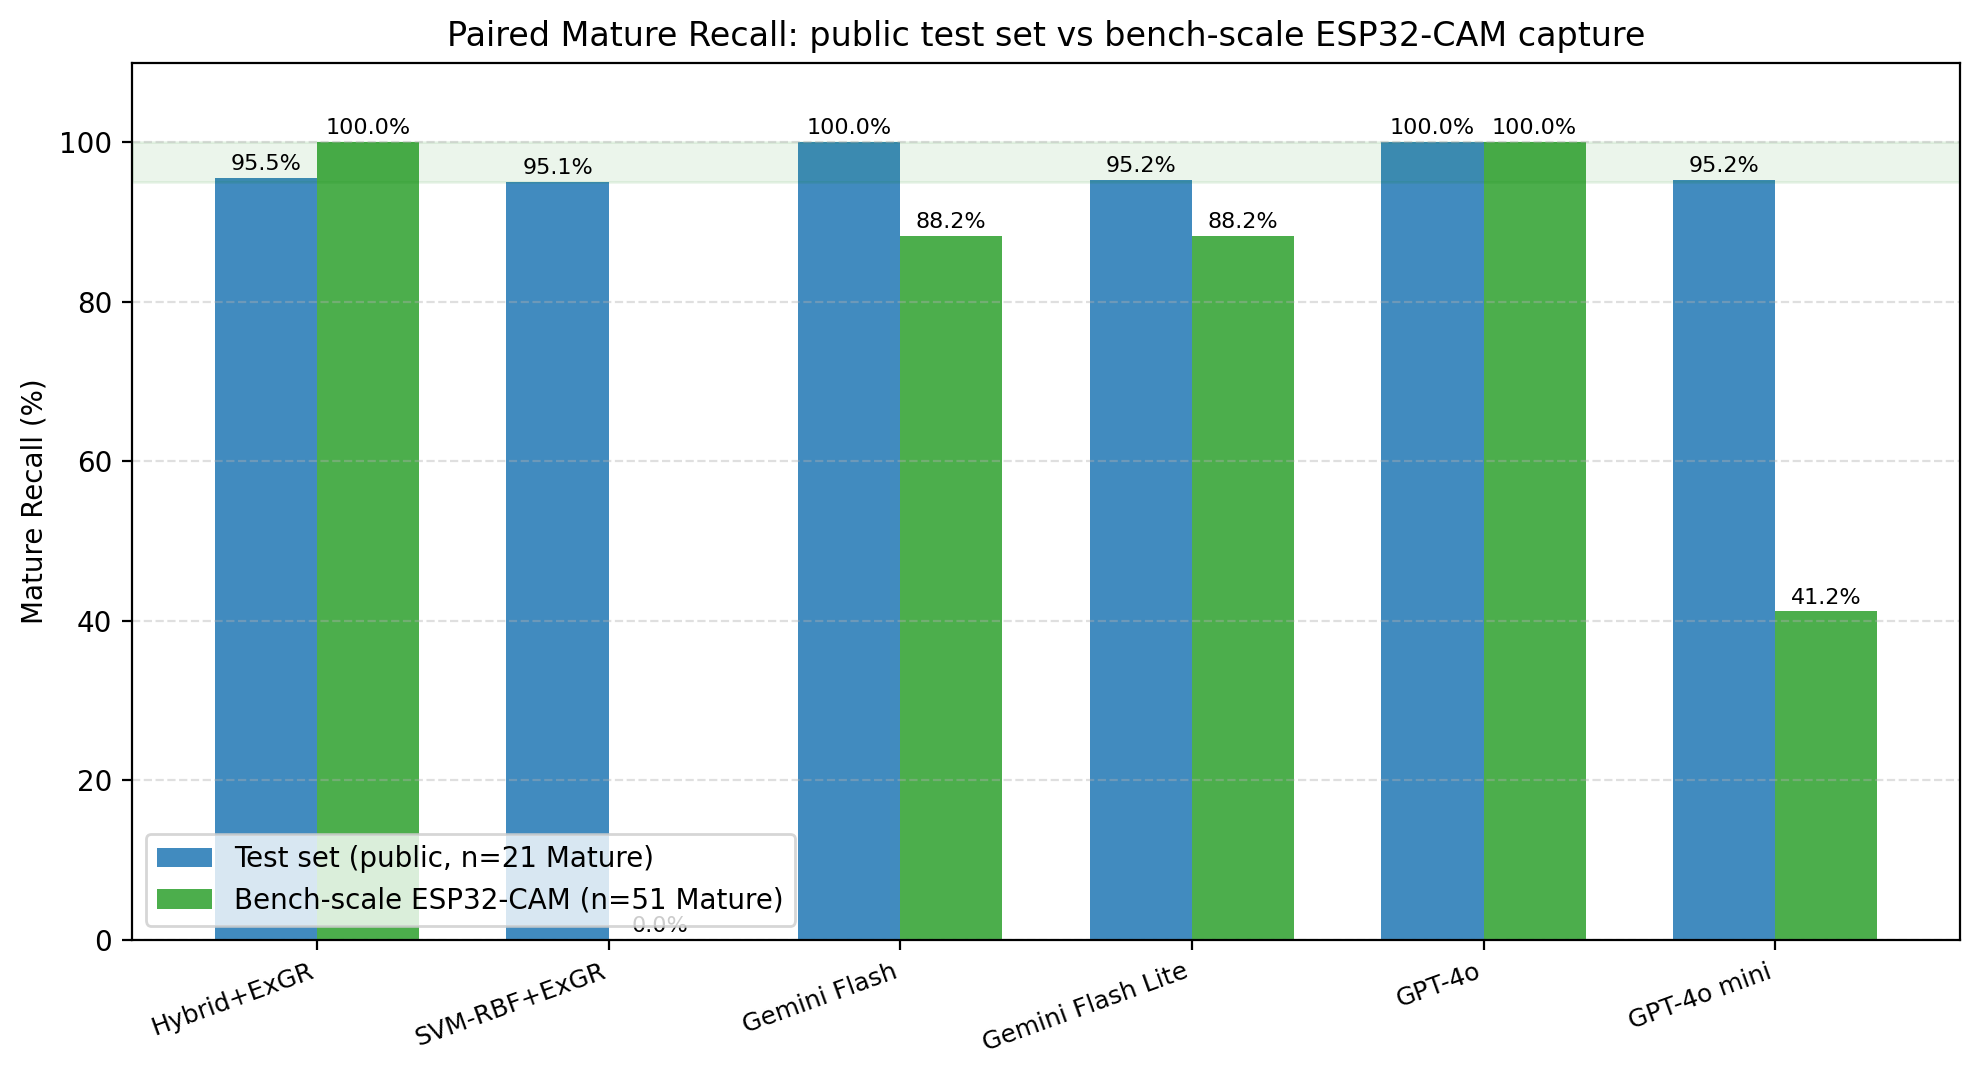
\includegraphics[width=0.85\textwidth]{img/Fig 4.5.3 Domain Shift.png}
    \caption{Mature Recall Delta: Curated vs ESP32-CAM Bench}
    \label{fig:domain-shift}
\end{figure}

\begin{figure}[H]
    \centering
    \includegraphics[width=0.85\textwidth]{img/Fig 4.5.3 VLM Rejections.png}
    \caption{ESP32-CAM Frames Rejected by GPT-4o Mini}
    \label{fig:vlm-rejections}
\end{figure}


% =============================================================
\section{Operational Cost}

The third comparative axis is operational cost, which decomposes into model artifact footprint, per-inference Cloud Run compute, and per-call vision-language API price. The Classical leader serializes to a $55$ KB joblib file, more than two orders of magnitude smaller than the $\sim$$17$ MB EfficientNetB0 SavedModel that backs both the Deep Learning leader and the Hybrid leader, and the footprint difference compounds at Cloud Run cold start because the tiny artifact loads on the first request without a perceptible delay while the EfficientNetB0 SavedModel measurably extends the wall-clock time that Cloud Run bills for. Cloud Run second-generation pricing in the Jakarta region charges per vCPU-second, per GiB-second of memory, and a fixed per-request component on a 1 vCPU and 512 MiB revision. The vision-language endpoints add a per-call billing layer that spans about $25$-fold within the vision-language cohort between Gemini 2.5 Flash Lite at $\sim$\$$0.045$ per thousand calls and GPT-4o at $\sim$\$$1.13$ per thousand calls under the structured prompt of about 250 input tokens and 50 output tokens, and more than two orders of magnitude relative to the Classical inference path.

\begin{table}[H]
    \centering
    \caption{Operational Cost Summary}
    \label{tab:cost-summary}
    \footnotesize
    \setlength{\tabcolsep}{4pt}
    \renewcommand{\arraystretch}{1.15}
    \begin{tabular}{@{}p{55mm}cp{45mm}r@{}}
        \hline
        Track / Endpoint & Artifact & Inference path & USD / 1k \\
        \hline
        Classical: SVM (RBF) + ExGR    & $55$ KB        & 18-dim $\rightarrow$ RBF kernel        & $\sim 0.003$  \\
        DL: EfficientNetB0             & $\sim 17$ MB   & $224{\times}224{\times}3$ CNN          & $\sim 0.005$  \\
        Hybrid: EfficientNetB0 + ExGR  & $\sim 17$ MB   & CNN(1280) + 18-dim concat              & $\sim 0.005$  \\
        VLM: Gemini 2.5 Flash Lite     & N/A            & HTTPS multimodal call                  & $\sim 0.045$  \\
        VLM: GPT-4o mini               & N/A            & HTTPS multimodal call                  & $\sim 0.068$  \\
        VLM: Gemini 2.5 Flash          & N/A            & HTTPS multimodal call                  & $\sim 0.20$   \\
        VLM: GPT-4o                    & N/A            & HTTPS multimodal call                  & $\sim 1.13$   \\
        \hline
    \end{tabular}
\end{table}

The classifier-only Cloud Run cost is derived from compute time on the order of $100$-$200$ ms per inference under the 1 vCPU and 512 MiB revision; differences between the three supervised tracks are below half a US cent per thousand calls and do not flip the ranking established by the accuracy metrics. The measured full-pipeline Cloud Run cost is larger because the gatekeeper LLM is invoked synchronously and Cloud Run bills for the wall-clock time the request handler is active. End-to-end measurement on the deployed Hybrid configuration with Gemini 2.5 Flash Lite as the gatekeeper gives a server-side median of $4006$ ms per inference, which translates to $\sim$\$$0.077$ per thousand calls of Cloud Run compute alone.

The deployed pipeline routes every capture through the vision-language gatekeeper before the supervised classifier, so the per-inference budget composes one gatekeeper call billed at the VLM rate plus one Cloud Run inference billed at compute time. With Gemini 2.5 Flash Lite as the gatekeeper and any of the three supervised tracks as the classifier, the per-thousand-inference budget is dominated by the synchronous gatekeeper wait and lands near $\$0.12$ per thousand calls. Replacing the gatekeeper with GPT-4o (the most expensive endpoint) raises the per-call cost by an order of magnitude on the VLM line item. The cost axis therefore favors keeping the cheaper Gemini tier on the gatekeeper side whenever Mature Recall is not the binding constraint, while the classifier choice on the supervised side is driven mainly by accuracy and cold-start footprint rather than per-inference compute cost.


% =============================================================
\section{Discussion}

Four threads run through the comparative results: the cross-validation versus test crossover inside the Hybrid track, the competitiveness of the Classical leader at a fraction of the Hybrid's artifact footprint, the zero-shot gap between vision-language endpoints and the supervised pool that justifies their reassignment to a gatekeeper role, and the data-governance consequences of choosing a lightweight versus a heavyweight classifier for the deployed pipeline.

\subsection{Hybrid: CV vs Test}

The NGRDI hybrid configuration leads the cross-validation pool at Macro F1 $0.9770$ but the ExGR hybrid configuration leads the test set at Macro F1 $0.9662$, a crossover of about $0.005$ on the primary metric between the two vegetation-index variants. With a test set of 104 images and a Mature subset of 21 images, the small-sample variance is large enough that the bootstrap 95\% intervals on the two configurations are expected to overlap substantially, and the crossover does not falsify the cross-validation ranking. The take-away for the comparative protocol is that paired bootstrap intervals are the right object to compare, not point-estimate ordinals.

\subsection{SVM-RBF as a Cheap Baseline}

The Classical leader (Support Vector Machine plus ExGR) lands at Macro F1 $0.9577$ on the test set, $0.0085$ below the Hybrid leader and $0.0045$ above the Deep Learning backbone, on a $55$ KB artifact against the $\sim$$17$ MB EfficientNetB0 pipeline and a single kernel evaluation rather than a convolutional forward pass through ImageNet-scale weights \cite{tanle2019efficientnet,sandler2018mobilenetv2}. On the curated test set this is an attractive trade: a negligible Macro F1 deficit for a two-orders-of-magnitude smaller cold-start footprint. The bench-scale result overturns it, since the same configuration collapses to $0.0000$ Mature Recall on the 51-frame ESP32-CAM set while the Hybrid holds at $1.0000$, so footprint alone cannot drive classifier selection.

\subsection{VLM Gap and Gatekeeper Role}

The vision-language zero-shot endpoints are not exposed to rice-stage supervision, so a Macro F1 deficit relative to the supervised pool is the expected outcome under the comparative protocol, and the open-set classification literature reports similar narrow-domain zero-shot gaps on agricultural imagery \cite{geng2021openset,zhang2024vlmsurvey,frontiers2026weedvlm}. The deficit observed here is narrower than expected at $0.025$ Macro F1 between Gemini 2.5 Flash Lite and the supervised Hybrid leader on the curated test set, but two findings keep the vision-language family out of the primary classifier role. Generative is systematically over-classified as Mature across all four tested endpoints, which is a class-pair confusion at the exact transition that the harvest-timing objective is most sensitive to. The bench-scale carry-over result then shows that the smaller endpoints drop sharply on ESP32-CAM imagery, with GPT-4o mini collapsing to $0.4118$ Mature Recall against a curated-test value of $0.9524$, while the supervised Hybrid configuration improves to perfect Mature Recall on the same bench captures. The gatekeeper role reassigns the vision-language endpoints to the task they natively support, deciding whether a frame is a plausible rice-canopy image at all, where all four endpoints reject every non-rice probe at zero false-accept rate.

\subsection{Deployment under Governance}

The comparative results convert the governance posture of the deployed pipeline into two operational levers that the operator can pull without redesigning the system. The first lever is model selection: the Classical leader (SVM-RBF plus ExGR) carries a $55$ KB joblib artifact more than two orders of magnitude smaller than the $\sim$$17$ MB EfficientNetB0 SavedModel that backs the Hybrid and Deep Learning leaders, so its per-event inference log satisfies the demonstrability requirement of Article 16(2)(h) of Law Number 27 of 2022 \cite{uupdp2022} against a smaller artifact footprint, a shorter Cloud Run warm window, and a narrower retention surface than any downstream Data Protection Impact Assessment would have to cover for the Hybrid configuration. That audit-surface advantage only matters for a classifier that works on the deployed sensor. The Classical configuration collapses to $0.0000$ Mature Recall on the ESP32-CAM bench set against $1.0000$ for the Hybrid configuration, so it does not. The deployed pipeline therefore keeps the Hybrid classifier regardless of audit surface, and the two configurations sit inside the same scoped-write and Cloud Logging envelope regardless of which one is active. The second lever is the architectural assignment of the vision-language model: the gatekeeper decision is a binary accept-or-reject on whether a frame is a plausible rice canopy at all, evidenced by the $0$ percent false-accept rate on the twelve non-rice probes, and that minimal decision concentrates the cross-border transfer surface to the smallest payload that the deployment has to send to a foreign-hosted endpoint under the third-country transfer provisions of Article 56 of Law Number 27 of 2022. Reassigning the vision-language model to the phenology classifier role, by contrast, would route every Vegetative, Generative, and Mature frame to the foreign endpoint and would enlarge the cross-border transfer surface by a factor equal to the capture cadence, which is the governance-side cost that the supervised classifier track avoids.

Table~\ref{tab:gov-crosswalk} crosswalks each regulatory and standards obligation against the architectural artifact that satisfies it and the empirical evidence from this chapter that quantifies the satisfaction. The crosswalk shows that the deployed pipeline discharges the national regime of Law Number 19 of 2016 \cite{uuite2016}, Government Regulation Number 71 of 2019 \cite{pp71_2019}, and Law Number 27 of 2022 alongside the international baseline of ITU-T Recommendation Y.2060 \cite{itut_y2060} and ISO/IEC 30141:2024 \cite{iso30141_2024} through a single set of artifacts rather than a parallel control set, and that the same artifacts already carry the audit evidence that an ISO/IEC 27001 or SNI ISO/IEC 27001 scoping exercise would consume, which makes the certification path a documentation step on top of the present deployment rather than a re-architecture step.

\begin{table}[H]
\centering
\caption{Regulation-to-Artifact-to-Evidence Crosswalk for the Deployed Pipeline}
\label{tab:gov-crosswalk}
\scriptsize
\renewcommand{\arraystretch}{1.2}
\setlength{\tabcolsep}{3pt}
\begin{tabularx}{\linewidth}{|>{\raggedright\arraybackslash}p{2.6cm}|>{\raggedright\arraybackslash}X|>{\raggedright\arraybackslash}X|>{\raggedright\arraybackslash}X|}
\hline
\textbf{Source} & \textbf{Obligation} & \textbf{Architectural artifact} & \textbf{Evidence} \\
\hline
UU 19/2016 & Integrity and authenticity of electronic information & Signed-URL upload binds each frame to verifiable provenance before inference & Latency log entries trace device, object, and prediction per capture \\
\hline
PP 71/2019 Art. 14 & Personal-data processing obligations for electronic system operators: purpose limitation, security protection, retention lifecycle, and breach notification & Identifier separation (device\_id path, no farmer token in object name), GCS lifecycle-delete rule on raw frames, and Cloud Logging for breach-event traceability & No farmer identifier appears in GCS object names or inference logs; lifecycle policy enforces deletion after retention window \\
\hline
UU 27/2022 Art. 16 & Data minimization, purpose limitation & Two separate RTDB trees for device identifiers and farmer identifiers with non-overlapping access rules & No analytical read path joins farmer identity to imagery in the inference logs \\
\hline
UU 27/2022 Art. 20 & Controller must establish and document a recognized lawful basis before processing personal data & Legitimate-interest basis (Art.~20(2)(f)) documented in system design; scoped Cloud Run IAM restricts inference calls to the declared agricultural-monitoring purpose & Per-event inference log records device identifier, predicted class, and model version, providing traceability evidence for the documented processing basis \\
\hline
UU 27/2022 Art. 56 & Third-country transfer minimization & Vision-language model used only as binary rice-or-not gatekeeper & $0$ percent false-accept on 12 non-rice probes; foreign endpoint sees only the smallest decision \\
\hline
ISO/IEC 30141:2024 & Cross-layer data protection (perception, network, application, security) & Scoped writes at perception, TLS at network, supervised classifier plus gatekeeper at application, IAM plus Cloud Logging at security & Latency budget decomposed across the four layers ($\sim$$3.7$ s WiFi, $\sim$$4$ s warm Cloud Run) \\
\hline
ITU-T Y.2060 & Interconnectivity, autonomic exchange, embedded security & Same scoped-write and structured-log surface as above & $8.57$ s end-to-end median latency under the warm-state cycle \\
\hline
\end{tabularx}
\end{table}

\subsection{Limitations}

The Mature class has support 21 on the test set, so the bootstrap interval on Mature Recall is wide (the Classical leader reports a 95\% interval of $[0.85, 1.00]$). Field validation is restricted to the Mature class on the bench-scale rig (four polybag-grown plants), so Vegetative and Generative performance on ESP32-CAM imagery has not been measured in this study and the carry-over result is single-class. The cross-validation pool is stratified at a Vegetative-Mature ratio near $1.10$, while the test set carries a ratio near $2.33$ by deliberate design as a robustness check; this stress-test setting is informative but the class-imbalance shift contributes to the small-sample noise visible in the cross-validation versus test crossover. The vision-language results reflect a single prompt design held constant across endpoints, so the systematic Generative-to-Mature confusion and the bench-scale rejection behavior of the smaller endpoints could be partially attributable to the prompt rather than to the models themselves, and a prompt-sensitivity study is left to future work. A larger Mature subset, a Vegetative or Generative bench-scale extension, and a prompt-design sweep across the four-endpoint cohort would tighten all four of these intervals.


% Bab 5: Kesimpulan dan Saran
%-----------------------------------------------------------------------------
\chapter{\babLima}
%-----------------------------------------------------------------------------

\section{Conclusions}

The four-family comparative study converges on a tight accuracy band under $95$ percent bootstrap confidence intervals: the Hybrid configuration pairing EfficientNetB0 with ExGR vegetation features leads test Macro F1 at $0.9662$, the classical SVM-RBF with ExGR follows at $0.9577$ in a $55$ KB artifact, and EfficientNetB0 alone reaches $0.9532$ on $104$ held-out images, with overlapping intervals that make the headline ordering not statistically separable at the present test-set size.

The vision-language cohort rejects all twelve non-rice probes at $0$ percent false-accept rate but collapses on phenology discrimination: it over-triggers Mature on Generative frames and fails on bench-scale carry-over, confirming that proprietary general-purpose endpoints are not viable as stand-alone phenology classifiers at this scale. The two-tier pipeline resolves the tension by assigning Gemini 2.5 Flash Lite as a binary gatekeeper at $4.81$ percent false-reject and placing the supervised Hybrid model as the phenology classifier behind it, achieving an end-to-end median latency of $8.57$ seconds inside the ten-minute capture cadence and $100$ percent Mature Recall on $51$ bench-scale frames.

Architectural assignment doubles as a regulatory compliance mechanism, though not through model selection: bench-scale validation showed the $55$ KB Classical artifact collapses to $0.0000$ Mature Recall on ESP32-CAM imagery against $1.0000$ for the deployed Hybrid configuration, so the compliance posture rests on where each component runs rather than on which supervised classifier is smallest. Hosting the supervised classifier in asia-southeast2 keeps personal data inside the jurisdiction whose protection regime governs it, and confining the vision-language model to a binary rice-or-not gate concentrates the cross-border transfer surface under Article 56 to the minimum decision the system must make. Together, this architectural assignment discharges the obligations of Law Number 19 of 2016, Government Regulation Number 71 of 2019, Law Number 27 of 2022, ISO/IEC 30141:2024, and ITU-T Recommendation Y.2060 within the deployed pipeline, independent of which supervised classifier is active behind the gatekeeper.


\section{Future Works}

Enlarging the Mature test subset beyond support $21$ would narrow the bootstrap interval on Mature Recall from its current $[0.85, 1.00]$ span and determine whether the $100$ percent bench-scale result holds across cultivar variation.

Extending the bench-scale rig to cover Vegetative and Generative frames and pairing it with a multi-device pilot on smallholder plots across cultivars, climates, and irrigation regimes would validate whether the latency and accuracy results transfer outside the controlled proximal-capture setup.

Replacing the proprietary gatekeeper with a self-hosted open-source vision-language model such as Qwen2.5-VL or InternVL2 on the same Cloud Run revision, combined with a Data Protection Impact Assessment under Law Number 27 of 2022 and an ISO/IEC 27001 or SNI ISO/IEC 27001 audit on the cloud backend, would close the cross-border transfer surface left open by the current deployment and evidence operator obligations under Government Regulation Number 71 of 2019 through external verification.

Quantizing MobileNetV3-Small for on-device inference through TensorFlow Lite Micro would push the classifier back onto the perception layer, eliminate the WiFi-side round trip that currently dominates the latency budget, and enable harvest-readiness detection without network connectivity.



% Daftar Referensi
\bibliographystyle{IEEEtran}
\bibliography{ref_database}
\clearpage

% Lampiran
\appendix
% Override ta.sty's \thetable/\thefigure/\thesection which hard-code
% \arabic{chapter}, so appendix items render as A.1, B.1 (using \thechapter)
% rather than colliding with body 1.1, 2.1.
\renewcommand{\thetable}{\thechapter.\arabic{table}}
\renewcommand{\thefigure}{\thechapter.\arabic{figure}}
\renewcommand{\thesection}{\thechapter.\arabic{section}}
% Singular "Appendix" instead of the appendix-package default "Appendices".
\renewcommand{\appendixname}{Appendix}
\include{./lampiran_A}
%\includepdf[pages=-]{lampiran/paper.pdf}
%\includepdf[pages=-]{lampiran/slide.pdf}


% Akhir bagian dari penulisan Laporan Tugas Akhir
\end{document}

%-----------------------------------------------------------------------------